\documentclass[12pt,letterpaper]{article}
\usepackage[utf8]{inputenc}
\usepackage[spanish]{babel}
\usepackage{amsmath}
\usepackage{color}
\usepackage{subcaption}
\usepackage{amsfonts}
\usepackage[colorlinks=true]{hyperref}
\usepackage{amssymb}
\usepackage{listings}

\usepackage{amsthm}
\newtheorem{theorem}{Teorema}

\usepackage{graphicx}
\usepackage[left=2cm,right=2cm,top=2cm,bottom=2cm]{geometry}
\setlength{\parskip}{3mm}
\title{\textsc{Distribución exponencial y de Poisson}}
\author{\textsc{Fabiola Vázquez}}

\setlength{\parindent}{0cm}

\begin{document}
\maketitle

\hrule
\section{Introducción}
Los objetivos de este estudio, que se realiza con el software estadístico R versión 4.0.2 \cite{R} en el IDE \textbf{R Studio} \cite{rstudio}, son encontrar relaciones entre las distribuciones exponencial y uniforme con la distribución de Poisson con algún parámetro $\lambda$. Siguiendo con el análisis de la novela \textit{Alice's Adventures in Wonderland} \cite{alice}, un objetivo más es encontrar algún dato, palabra, frase, longitud, etcétera, que siga una distribución de Poisson.  

\section{Uso de la distribución exponencial}
En el primer estudio, se generan números distribuidos exponencialmente con parámetro \texttt{lambda} y se calcula la cantidad necesaria para que su suma exceda a una \texttt{meta}. Dicho proceso, se realiza una cierta cantidad de veces. El objetivo es ver si esos números que se producen y guardan en el vector \texttt{ce} se distribuyen Poisson con algún parámetro $\lambda$, el algoritmo fue realizado por la Dra. Elisa Schaeffer.


\begin{lstlisting}[frame=single]
for (replica in 1:replicas) {
    de = numeric()
    
    while (sum(de) < meta) {
        de = c(de, rexp(1, lambda))
    }
    ce = c(ce, length(de)-1)
}
\end{lstlisting}

La media de la distribución exponencial es $\frac{1}{\lambda}$ \cite{casella}. Se sabe que la distribución de Poisson tiene como parámetro $\lambda$ que es la tasa de llegadas en un intervalo de tiempo \cite{elisaproba}. Entonces, \textbf{se espera} que la tasa de llegadas sea de \texttt{meta}$\cdot$\texttt{lambda}.

Se realiza unas pruebas, para ver si se va por buen camino, variando los valores de los parámetros \texttt{meta} y \texttt{lambda}. En la figura \ref{prs} se compara el histograma de los números generados, lado izquierdo, contra el histograma de valores generados con \texttt{rpois(replica,me*la)}, lado derecho. Visualmente los histogramas son idénticos.



\begin{figure}
 	\centering 
 	\begin{subfigure}[b]{0.45\linewidth}
 		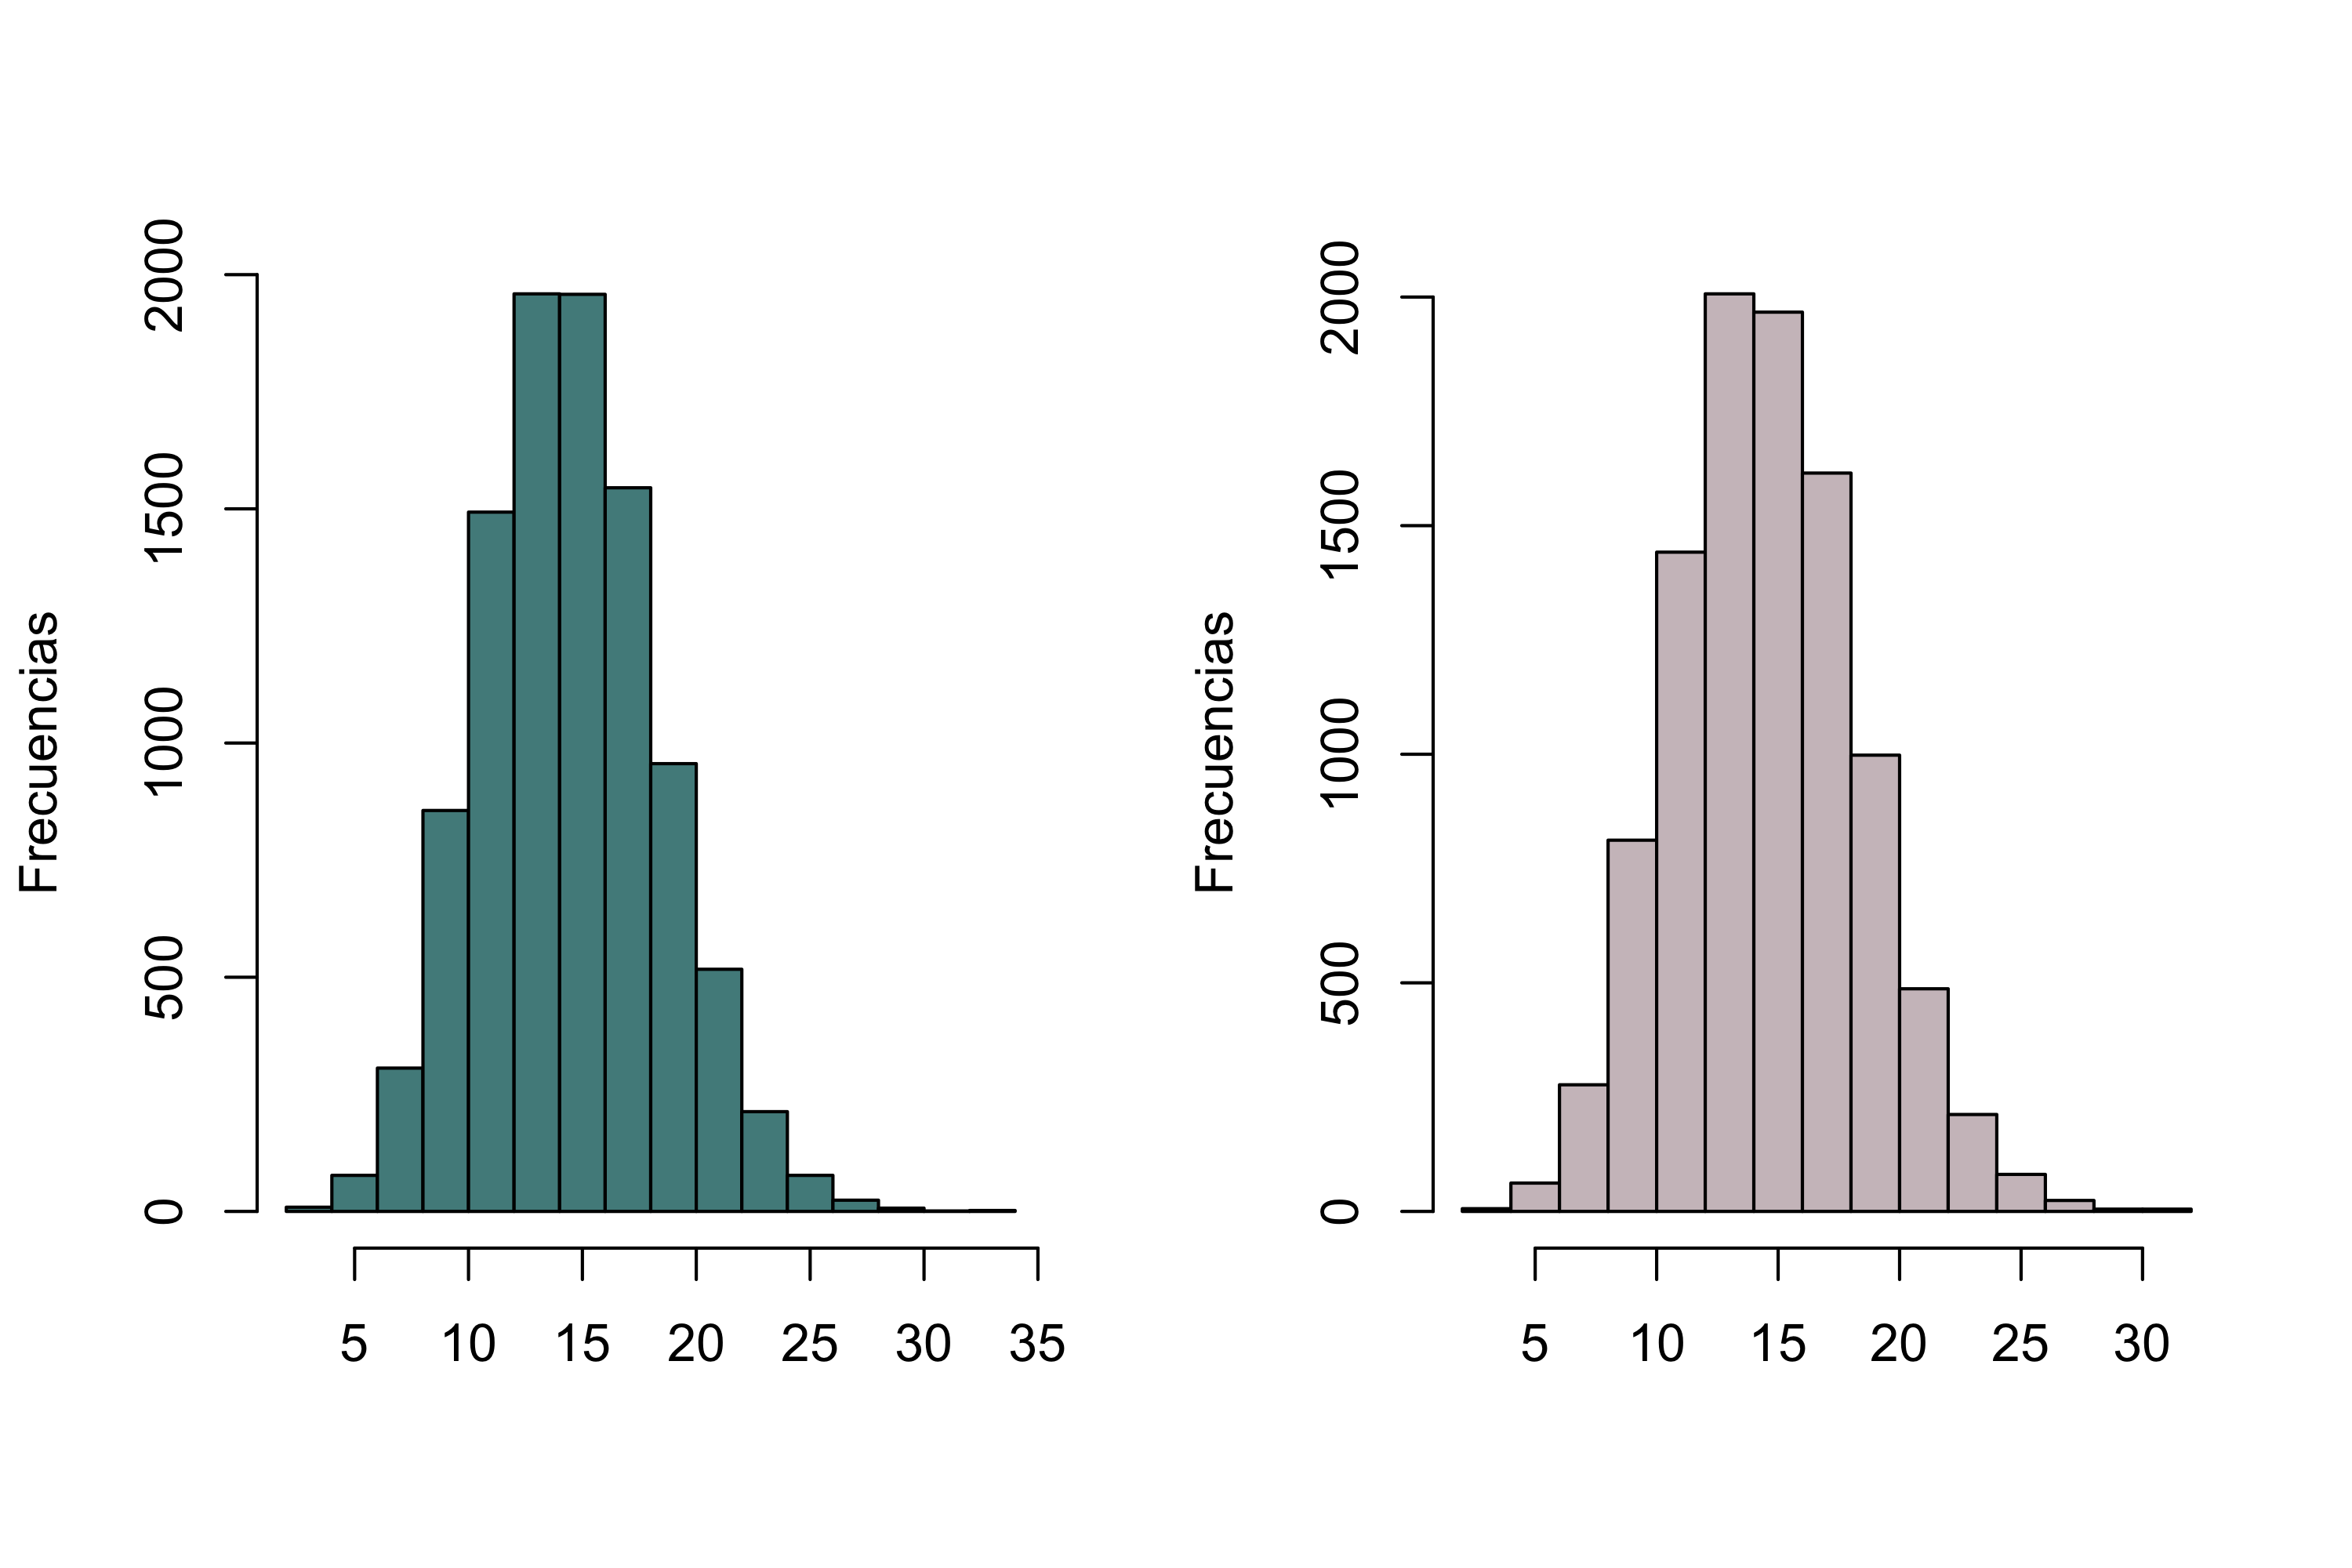
\includegraphics[width=\linewidth]{prueba1.png} 		
 		\caption{Números generados con \texttt{meta}=3 y \texttt{lambda}=5 (izq) contra los generados con \texttt{rpois} (der).}
 		 		\label{pr1}
 	\end{subfigure}
 	\hfill
 	\begin{subfigure}[b]{0.45\linewidth}
 		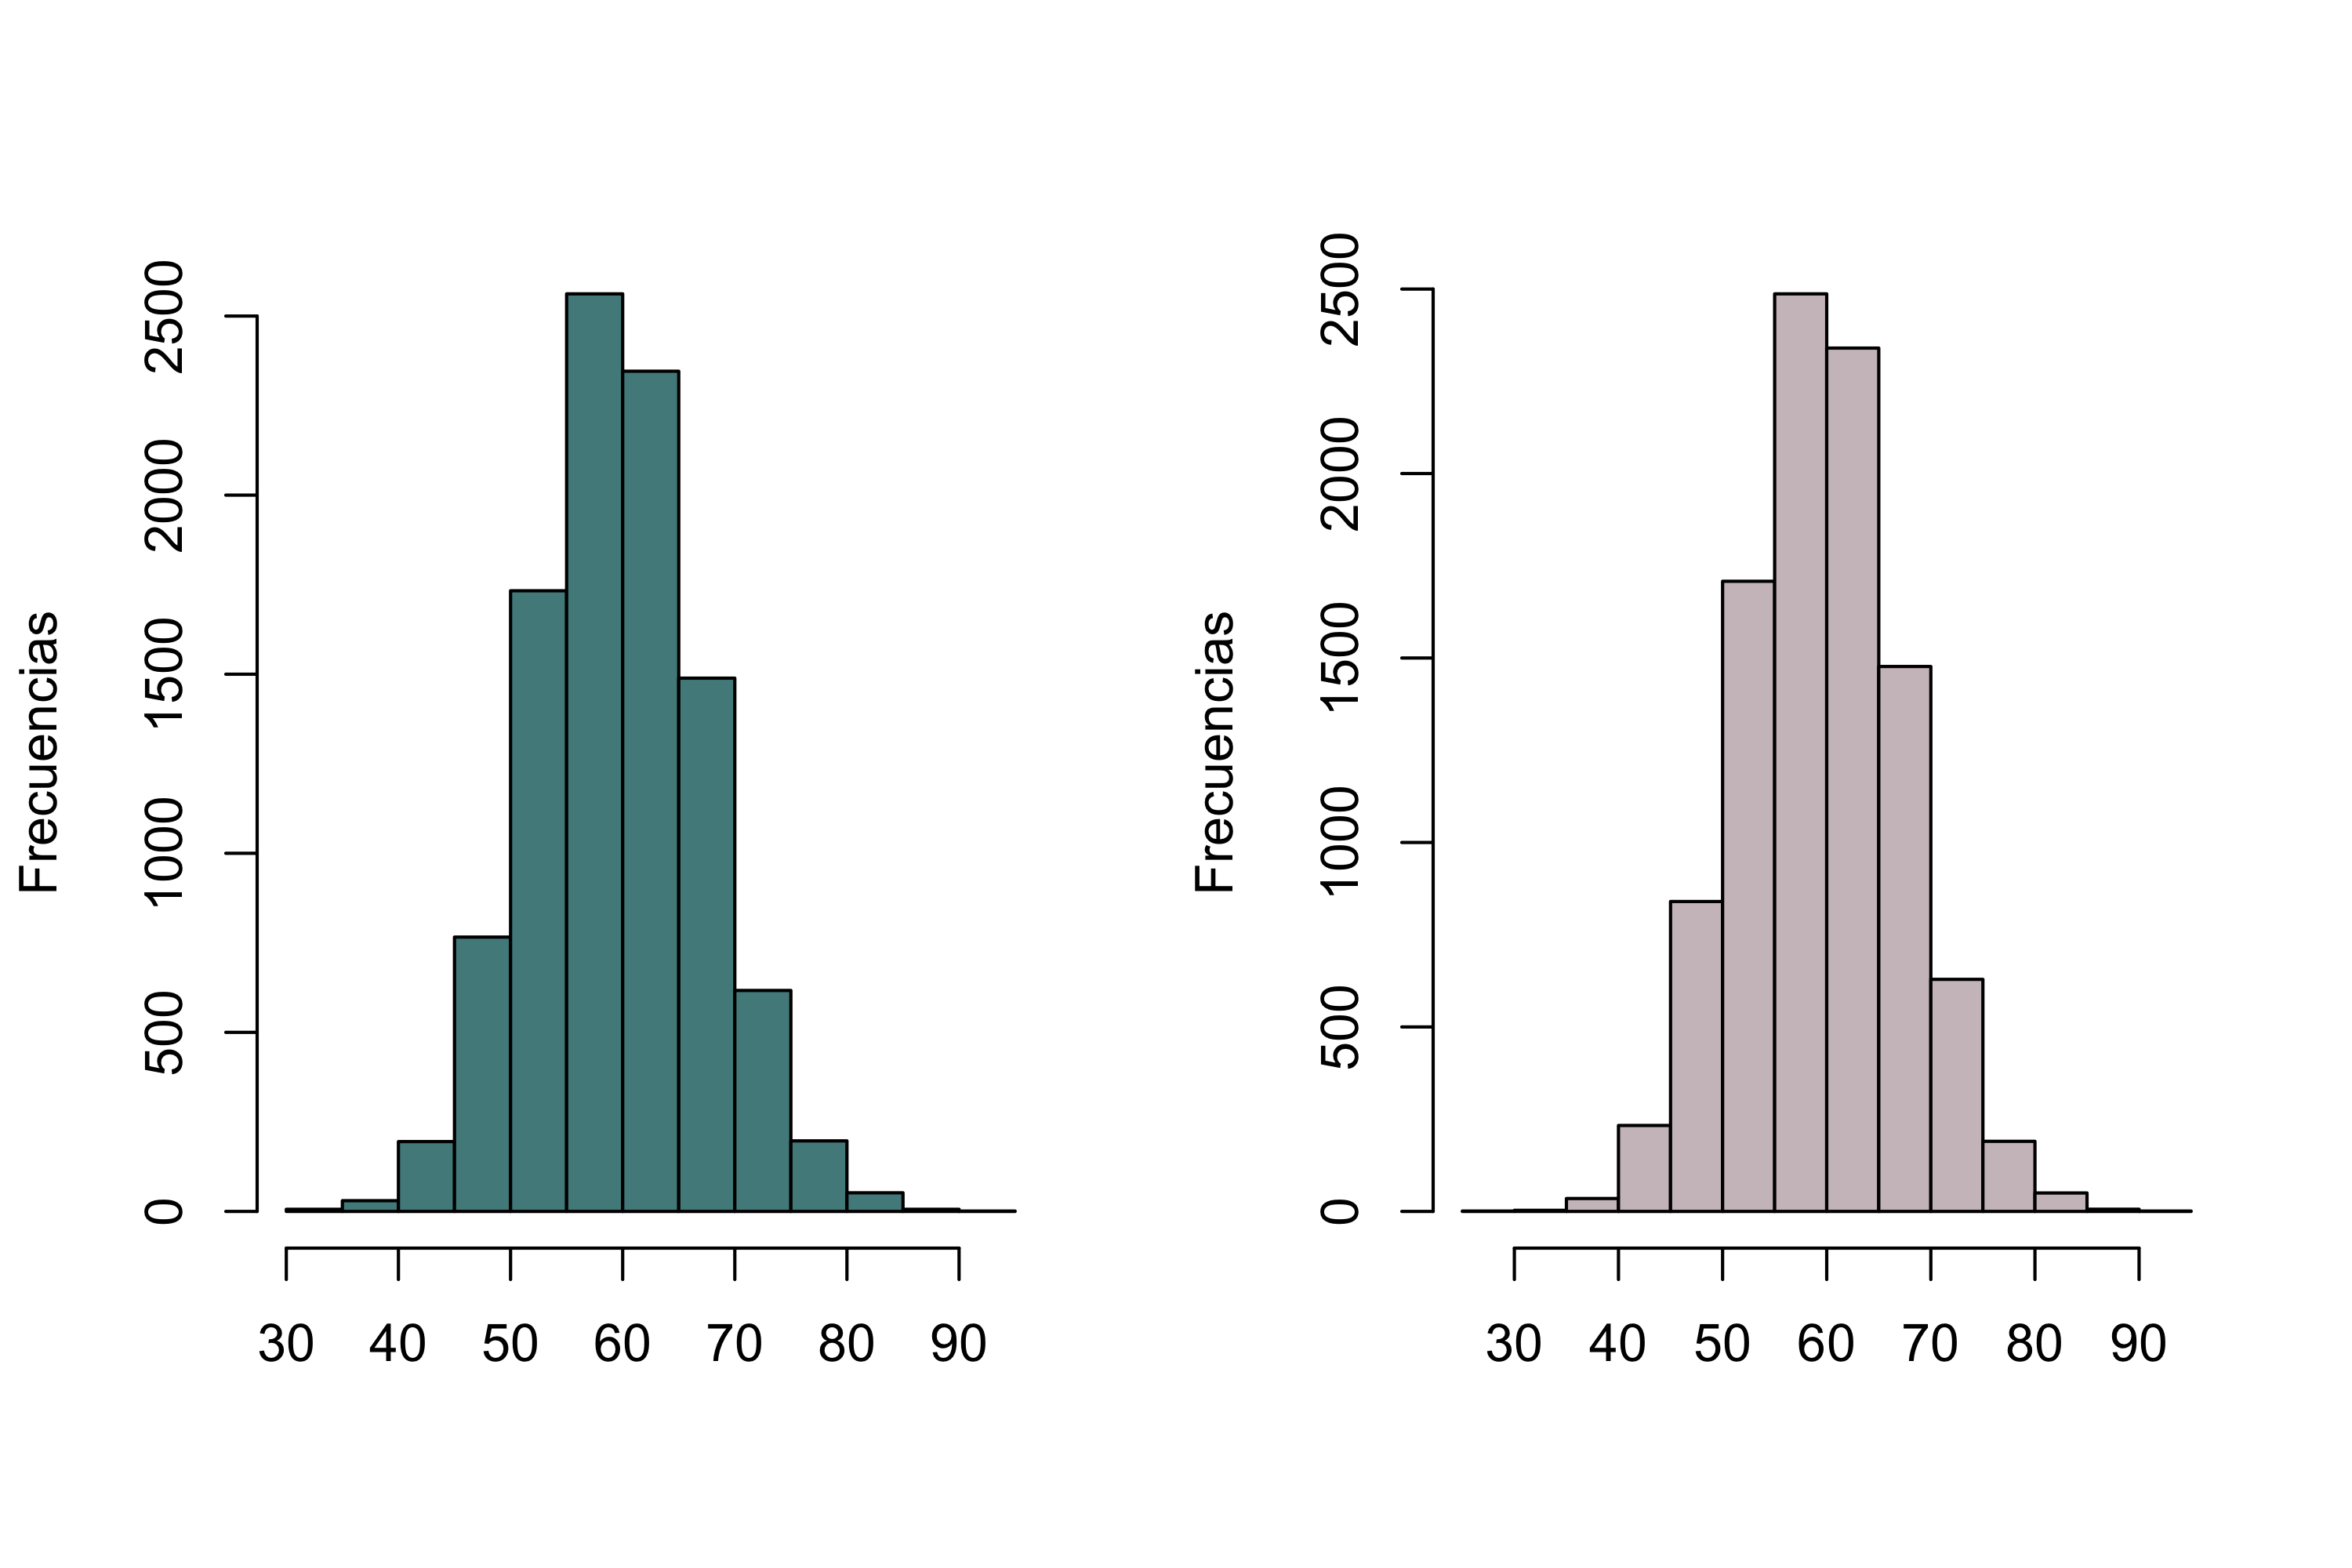
\includegraphics[width=\linewidth]{prueba2.png} 		
 		\caption{Números generados con \texttt{meta}=10 y \texttt{lambda}=6 (izq) contra los generados con \texttt{rpois} (der).}
 		\label{pr2}
 	\end{subfigure}
 	 	\begin{subfigure}[b]{0.45\linewidth}
 		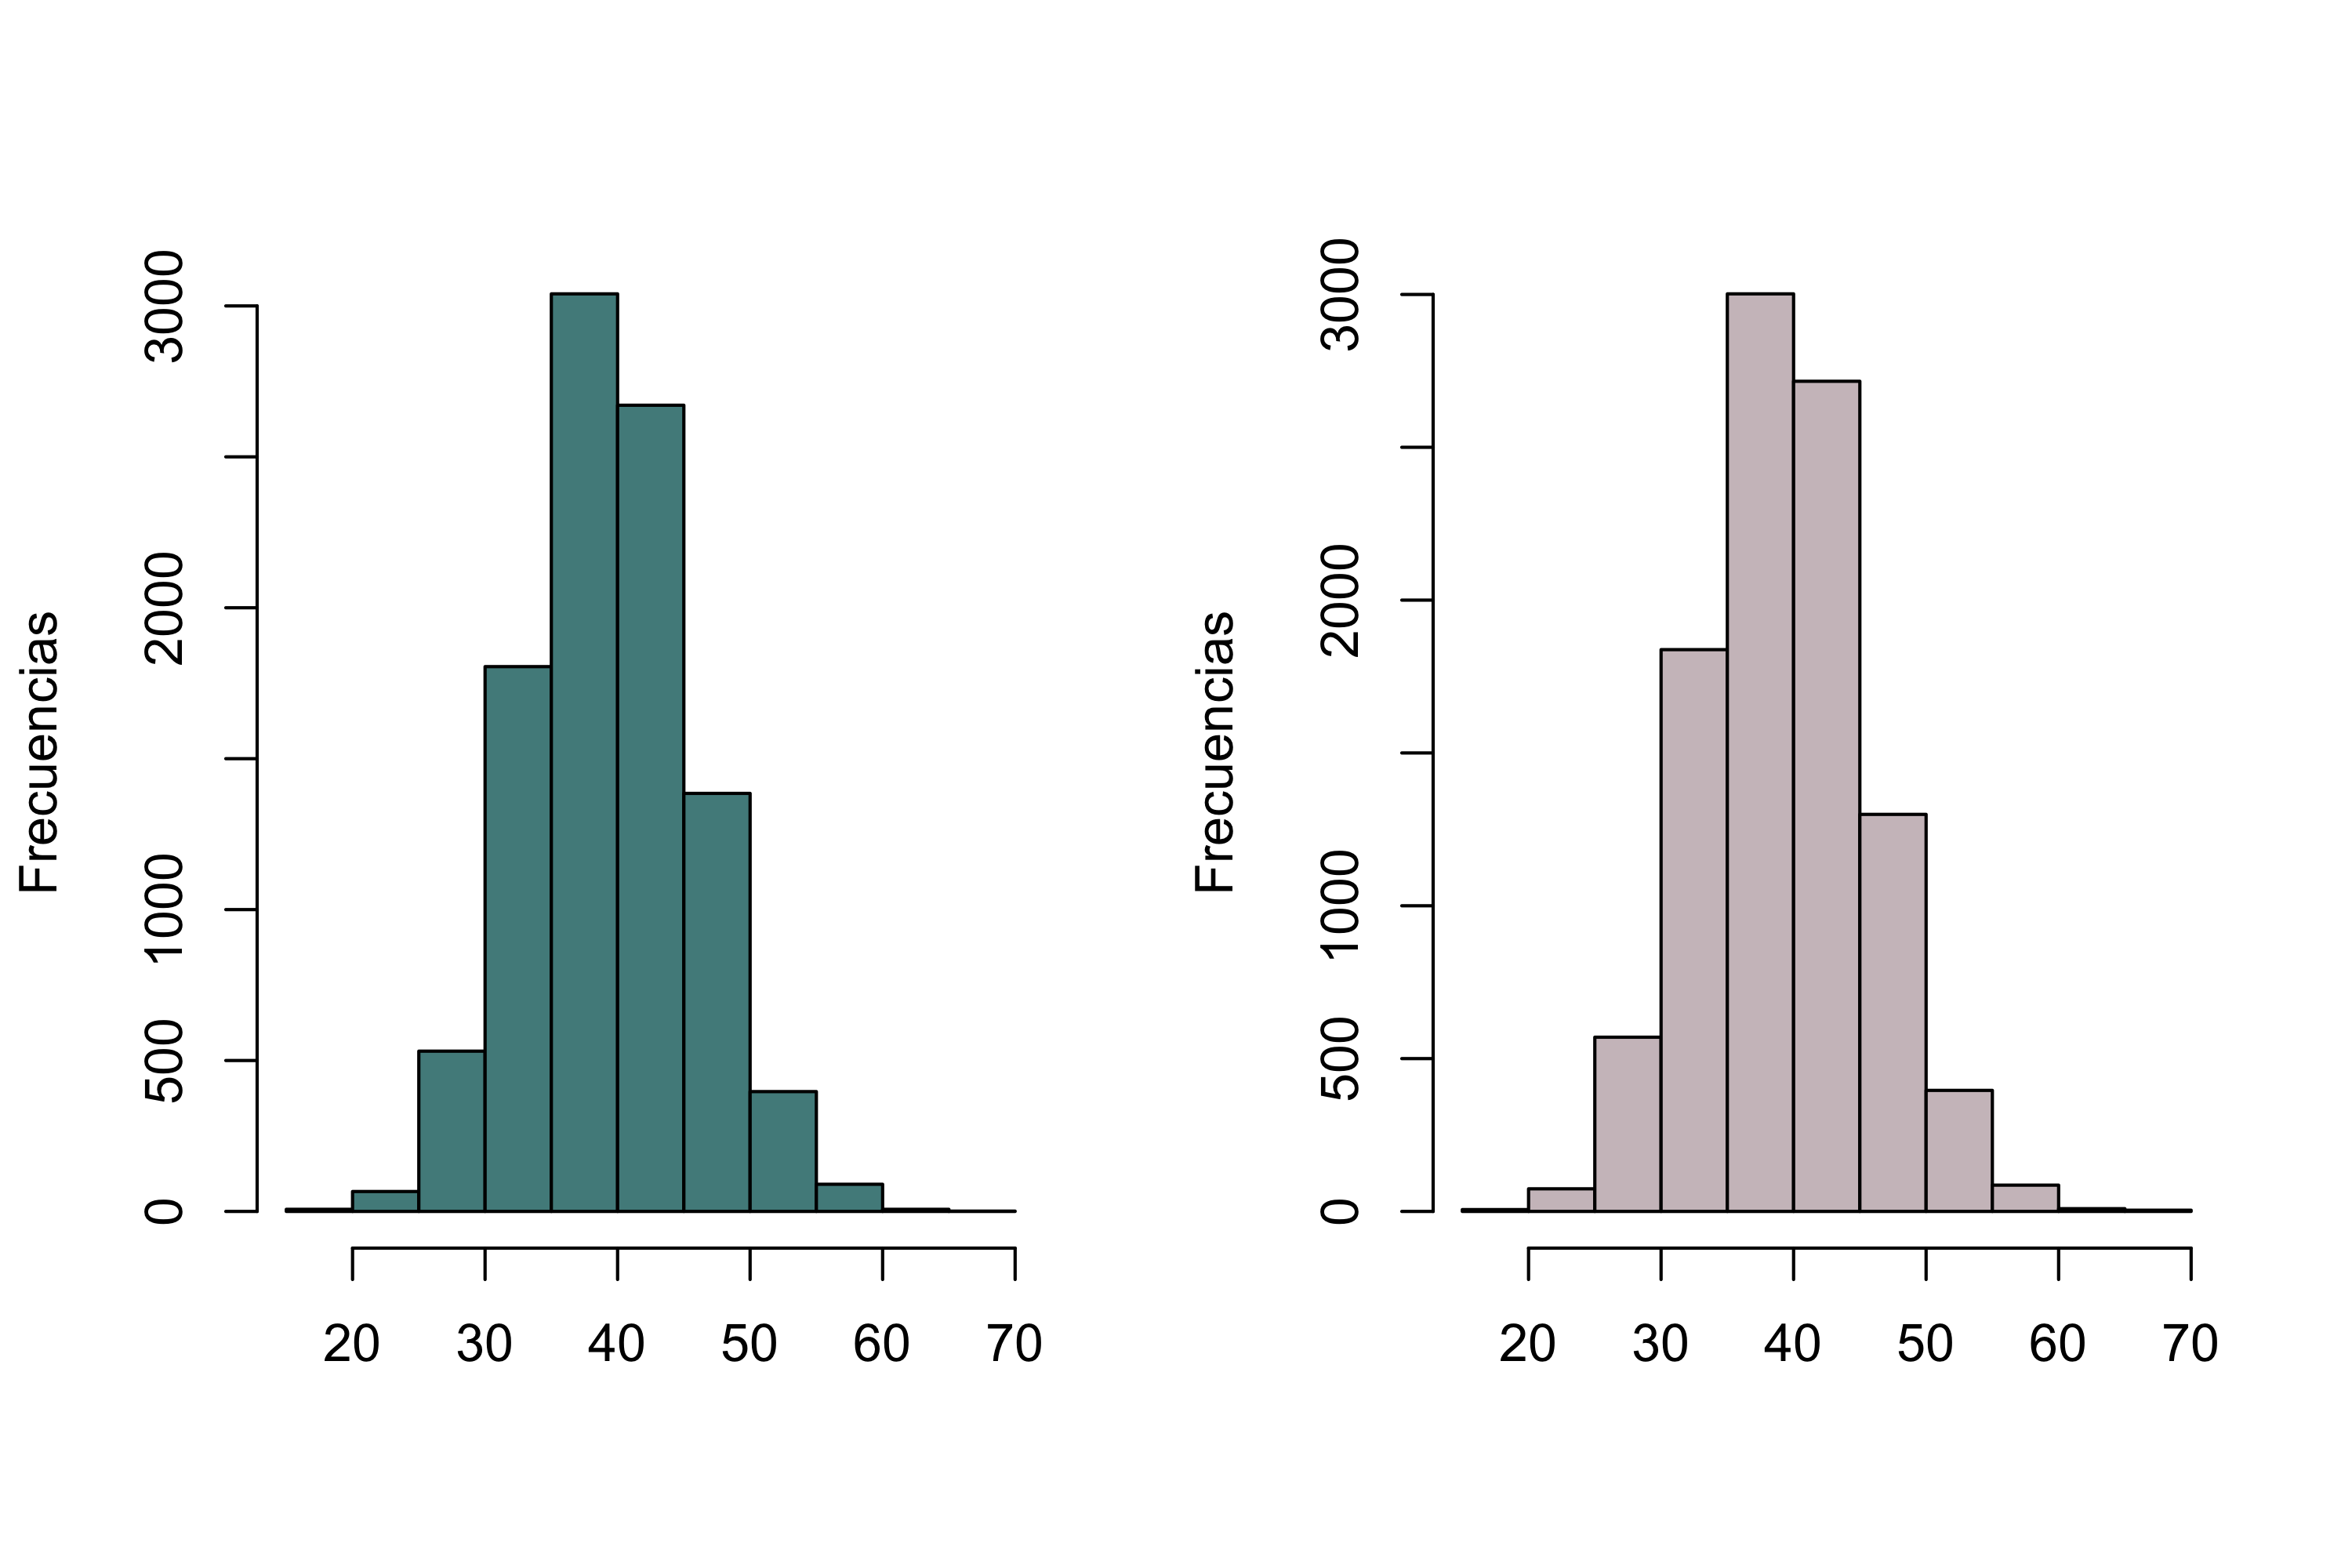
\includegraphics[width=\linewidth]{prueba3.png} 		
 		\caption{Números generados con \texttt{meta}=4 y \texttt{lambda}=10 (izq) contra los generados con \texttt{rpois} (der).}
 		\label{pr3}
 	\end{subfigure}
 	 	\hfill
 	 	\begin{subfigure}[b]{0.45\linewidth}
 		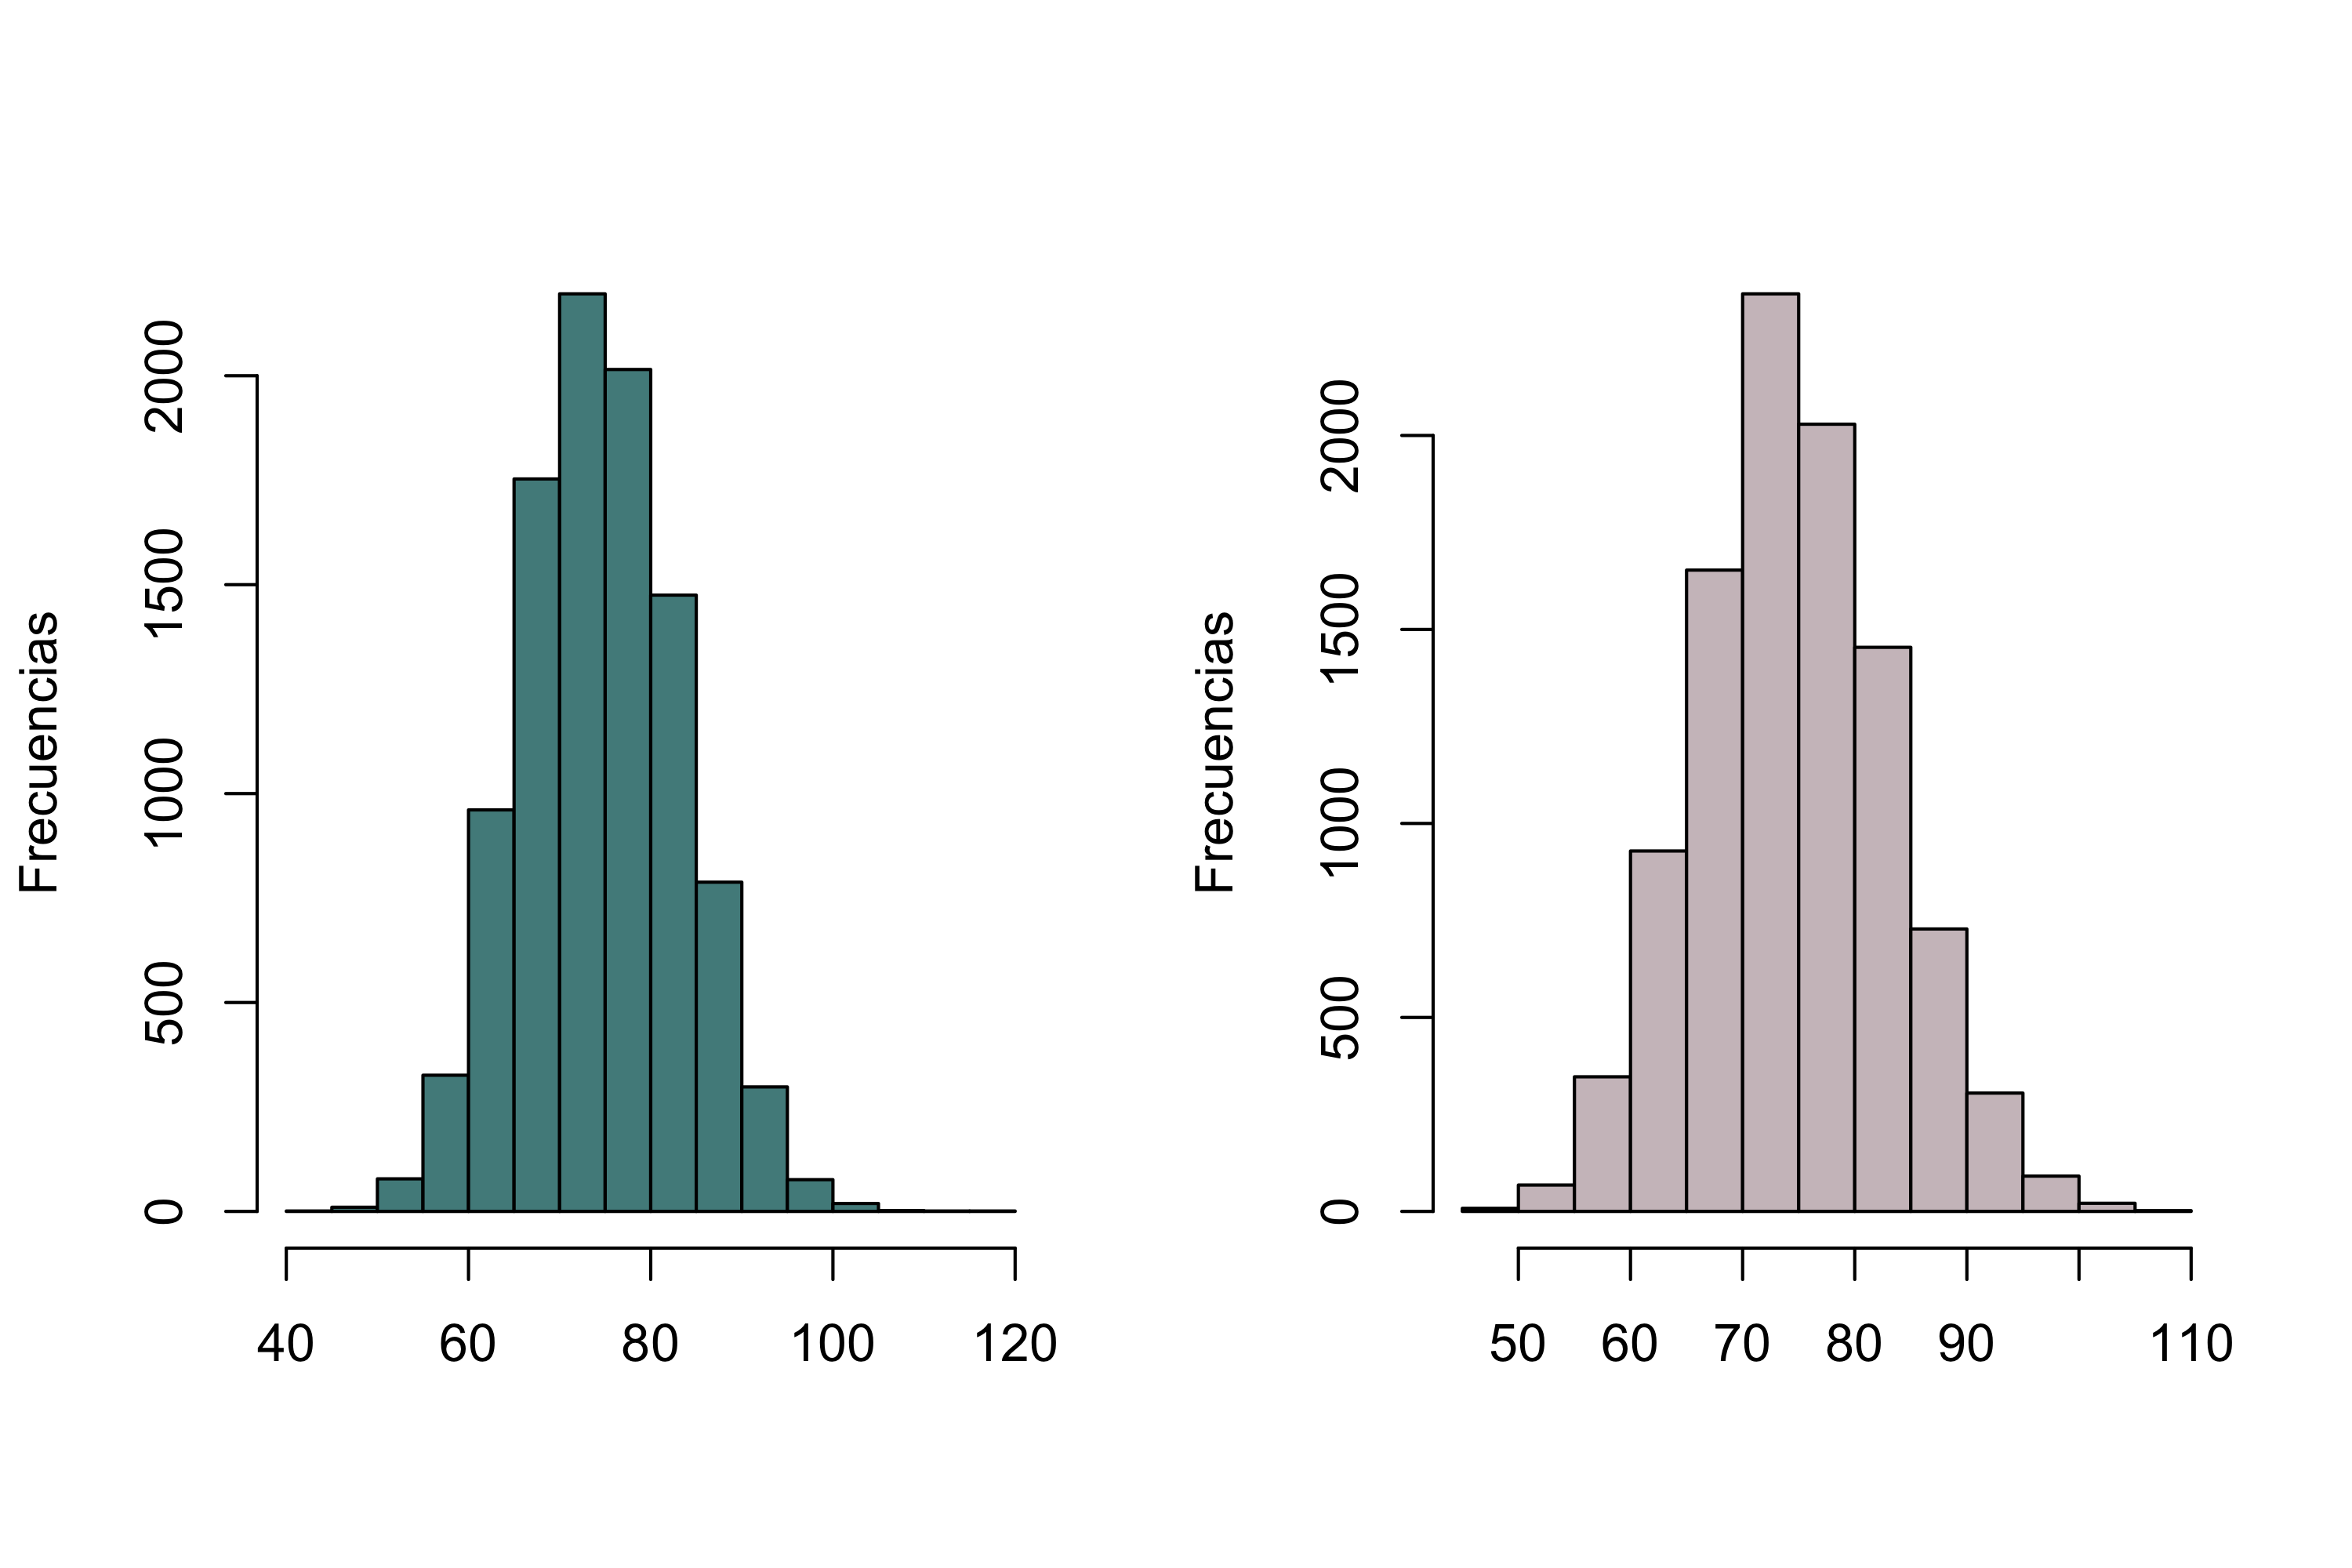
\includegraphics[width=\linewidth]{prueba4.png} 		
 		\caption{Números generados con \texttt{meta}=15 y \texttt{lambda}=5 (izq) contra los generados con \texttt{rpois} (der).}
 		\label{pr4}
 	\end{subfigure}

 	 	\caption{Pruebas usando el algoritmo para crear números distribuidos Poisson.} 
 	 		\label{prs}
\end{figure}
Se utiliza la función \texttt{goodfit} del paquete \texttt{vcd} para hacer una prueba de bondad de ajuste Chi cuadrada, para analizar si el conjunto de datos generados se distribuye de forma Poisson. La función nos regresa también el valor del parámetro $\lambda$ necesario. 


\begin{table}
\centering
\caption{Comparación de los parámetros usados y el lambda dado por \texttt{goodfit}.}
\begin{tabular}{cccr}
\hline 
Prueba & Meta & Lambda & Lambda (goodfit) \\ 
\hline 
1 & 3 & 5 & 15.019 \\ 
2 & 10 & 6 & 59.869 \\ 
3 & 4 & 10 & 39.982 \\ 
4 & 15 & 5 & 74.995 \\ 
\hline 
\end{tabular} 
\label{datos}
\end{table}

En el cuadro \ref{datos} se ve que en las pruebas realizadas, el valor obtenido mediante \texttt{goodfit} se asemeja, en efecto, al valor de \texttt{meta}$\cdot$\texttt{lambda}.

\begin{figure}
\centering
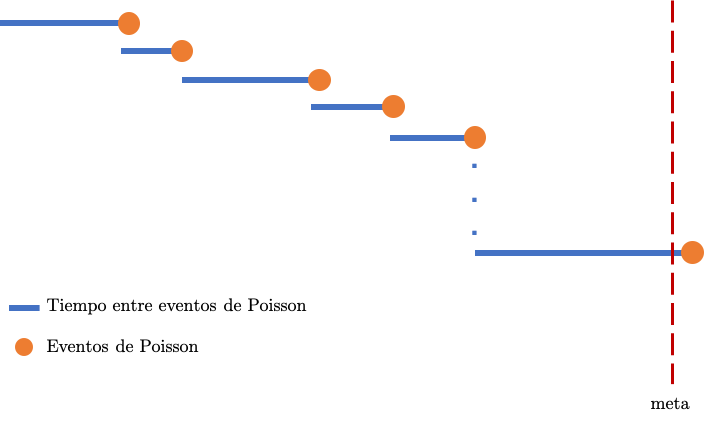
\includegraphics[width=9cm]{dibujo.png} 		
\caption{Visualización del experimento}
 \label{exp}

\end{figure}

Otra perspectiva al experimento, es ver que los números distribuidos exponencialmente que se generan son las diferencias entre los eventos de Poisson, como se ve en la figura \ref{exp}. 

\begin{theorem}
El tiempo necesario para que ocurra el primer evento de Poisson tiene distribución exponencial, con parámetro $\lambda t$. 

\end{theorem}

\begin{proof}
Se considera que $X \sim $ Poisson($\lambda t$). La probabilidad de obtener $n$ llegadas en un intervalo, se obtiene como
 \begin{equation}
 P(X=n)=\frac{(\lambda t)^{n}}{n!}e^{-\lambda t}
 \end{equation}
Entonces, la probabilidad de que no haya llegadas en el intervalo sería

\begin{equation}
P(X=0)=e^{-\lambda t}
\end{equation}
La probabilidad de que $T$ exceda $x$ es la misma que la probabilidad de que no ocurra ningún evento de Poisson en $x$.

\begin{equation}
P(T> x) = e^{-\lambda t}
\end{equation}
Entonces,
\begin{equation}
P(T\leqslant x)=1-P(T> x) = 1-e^{-\lambda t}
\end{equation}
\end{proof}


 

\section{Uso de la distribución uniforme}
Se generan números distribuidos uniformemente y con el \textit{algoritmo de Knuth} \cite{Knuth} que calcula el producto de dichos números mientras sea mayor que \texttt{e**-lambda}, se guarda la cantidad de números. Se quiere ver si los números generados siguen una distribución de Poisson con parámetro \texttt{lambda.}


Se realizan pruebas variando los valores de \texttt{lambda}. Los histogramas se aprecian en la figura \ref{datosunif} y las comparaciones con los valores de \texttt{lambda} obtenidos con \texttt{goodfit} se encuentran en el cuadro \ref{datosunif}.
\begin{figure}
 	\centering 
 	\begin{subfigure}[b]{0.45\linewidth}
 		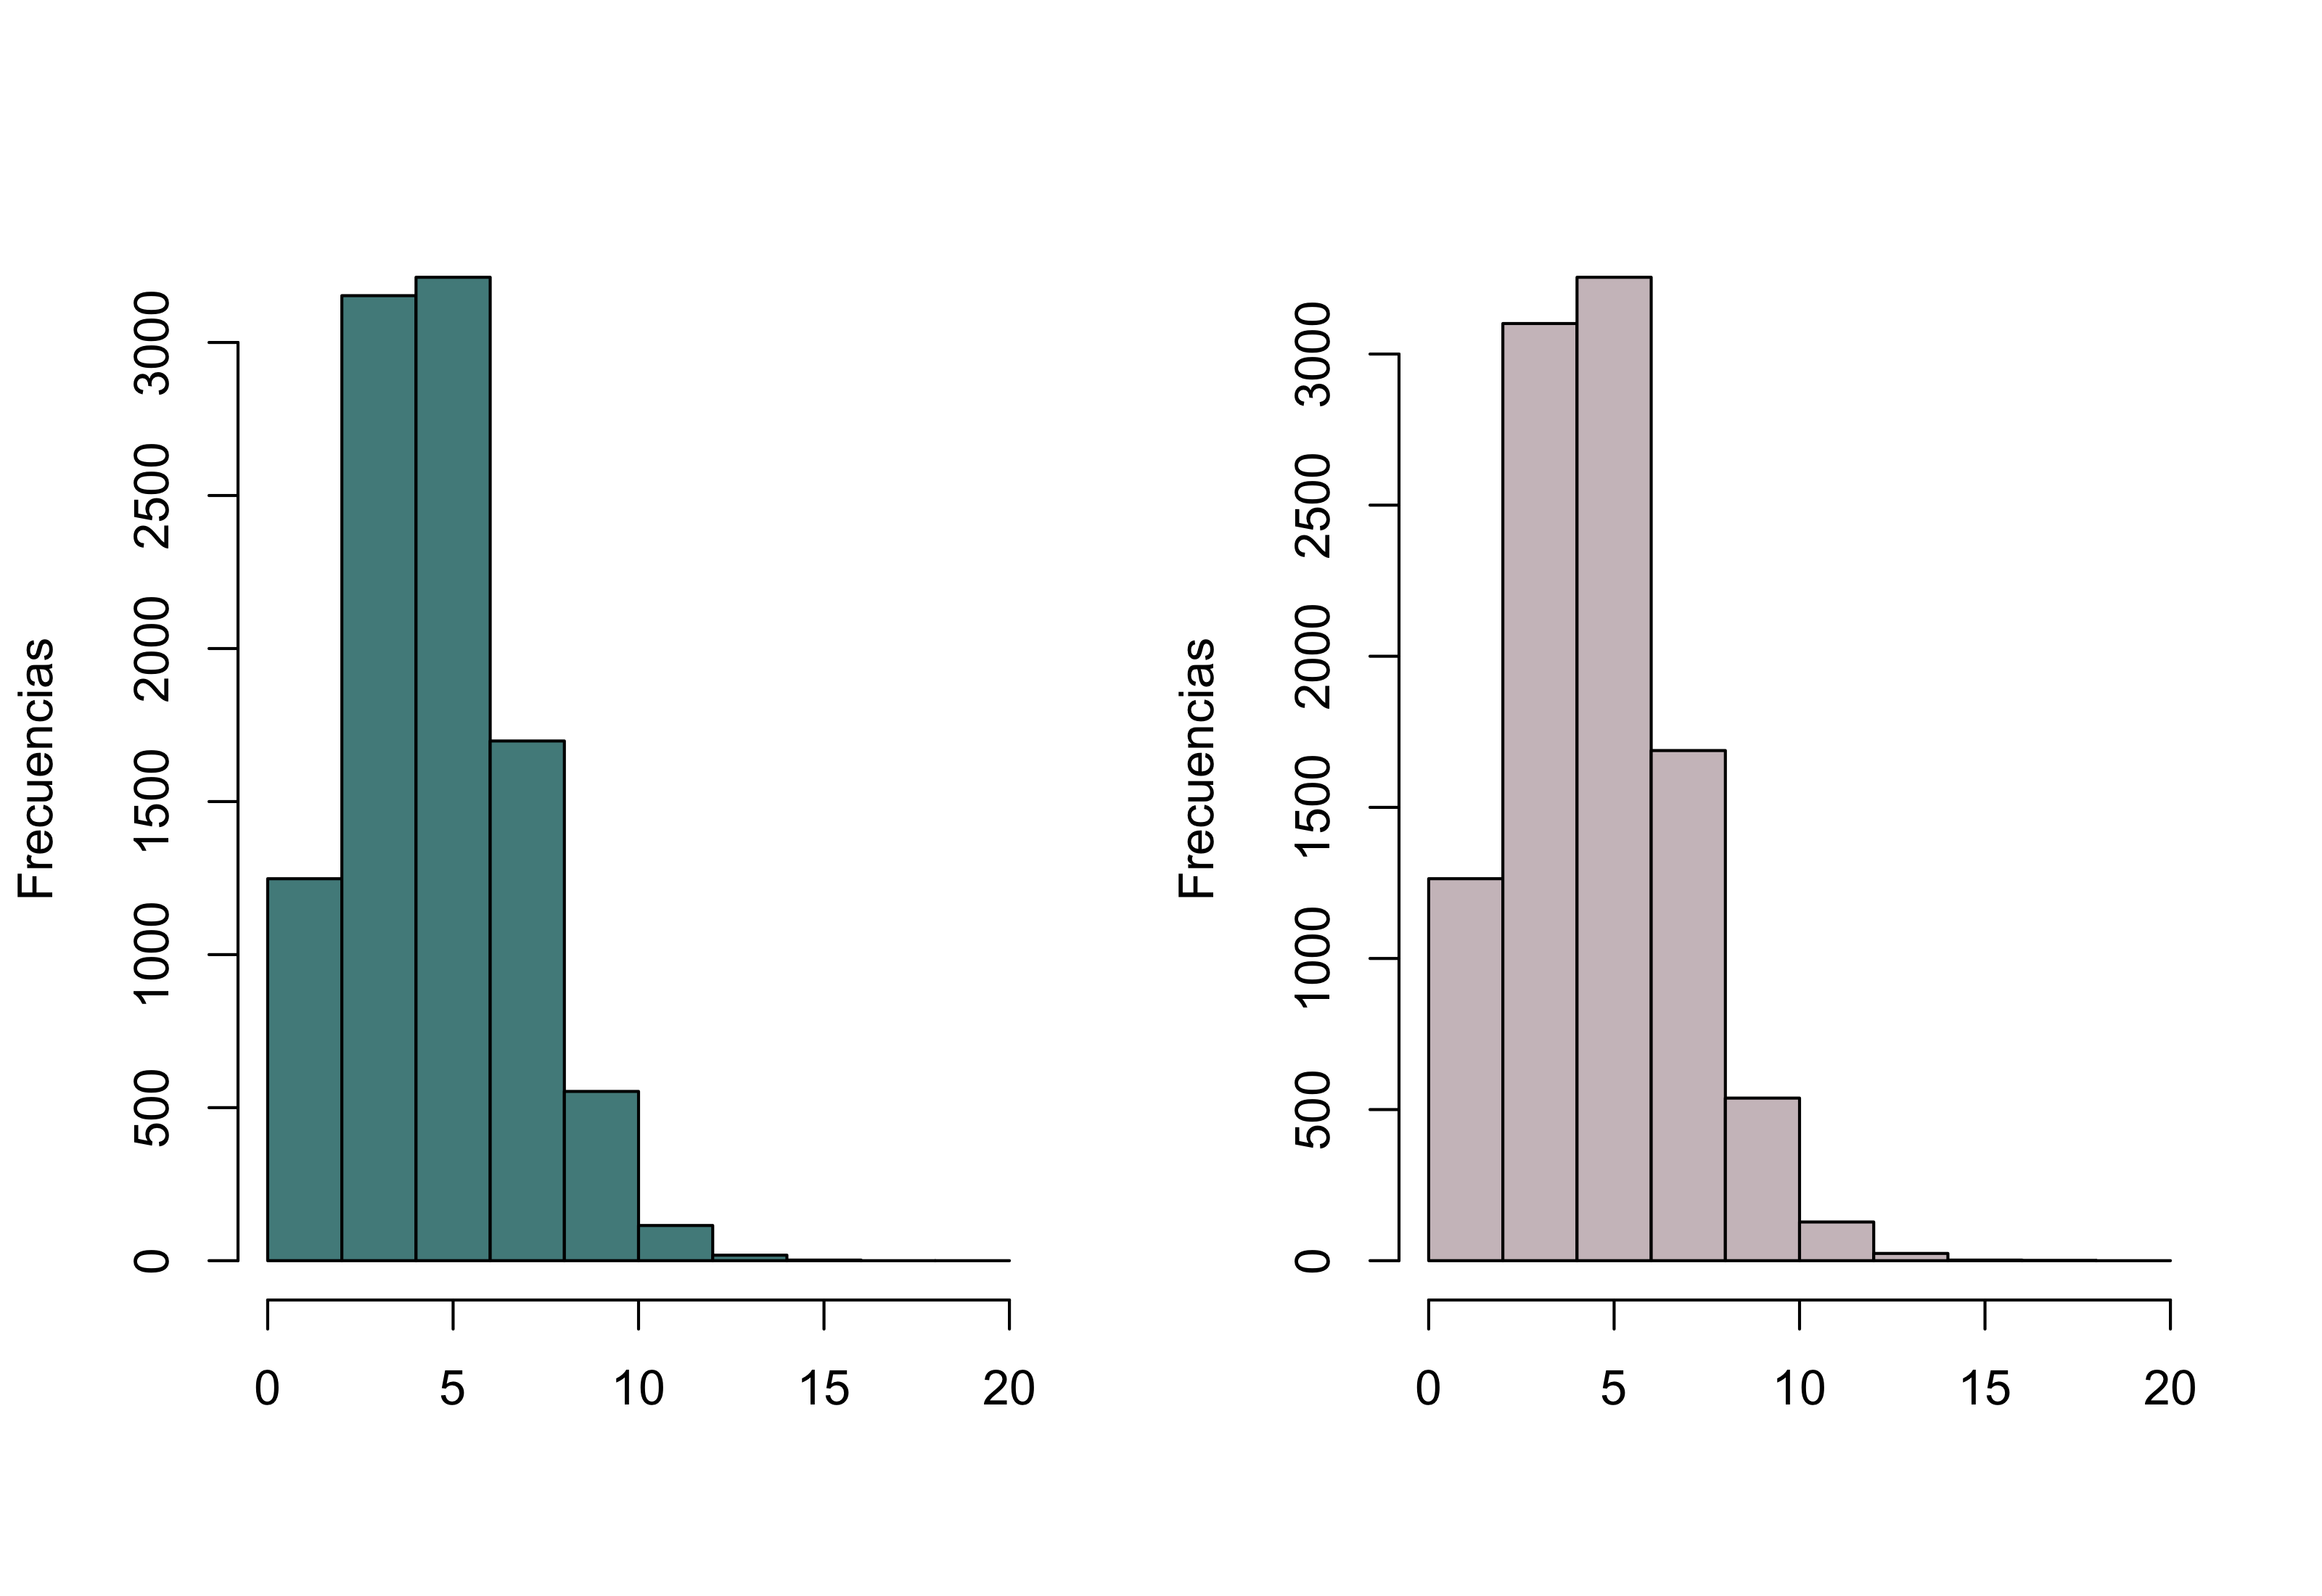
\includegraphics[width=\linewidth]{unif1.png} 		
 		\caption{Números generados con \texttt{lambda}=5 (izq) contra los generados con \texttt{rpois} (der).}
 		 		\label{pr1unif}
 	\end{subfigure}
 	 	\hfill
 	\begin{subfigure}[b]{0.45\linewidth}
 		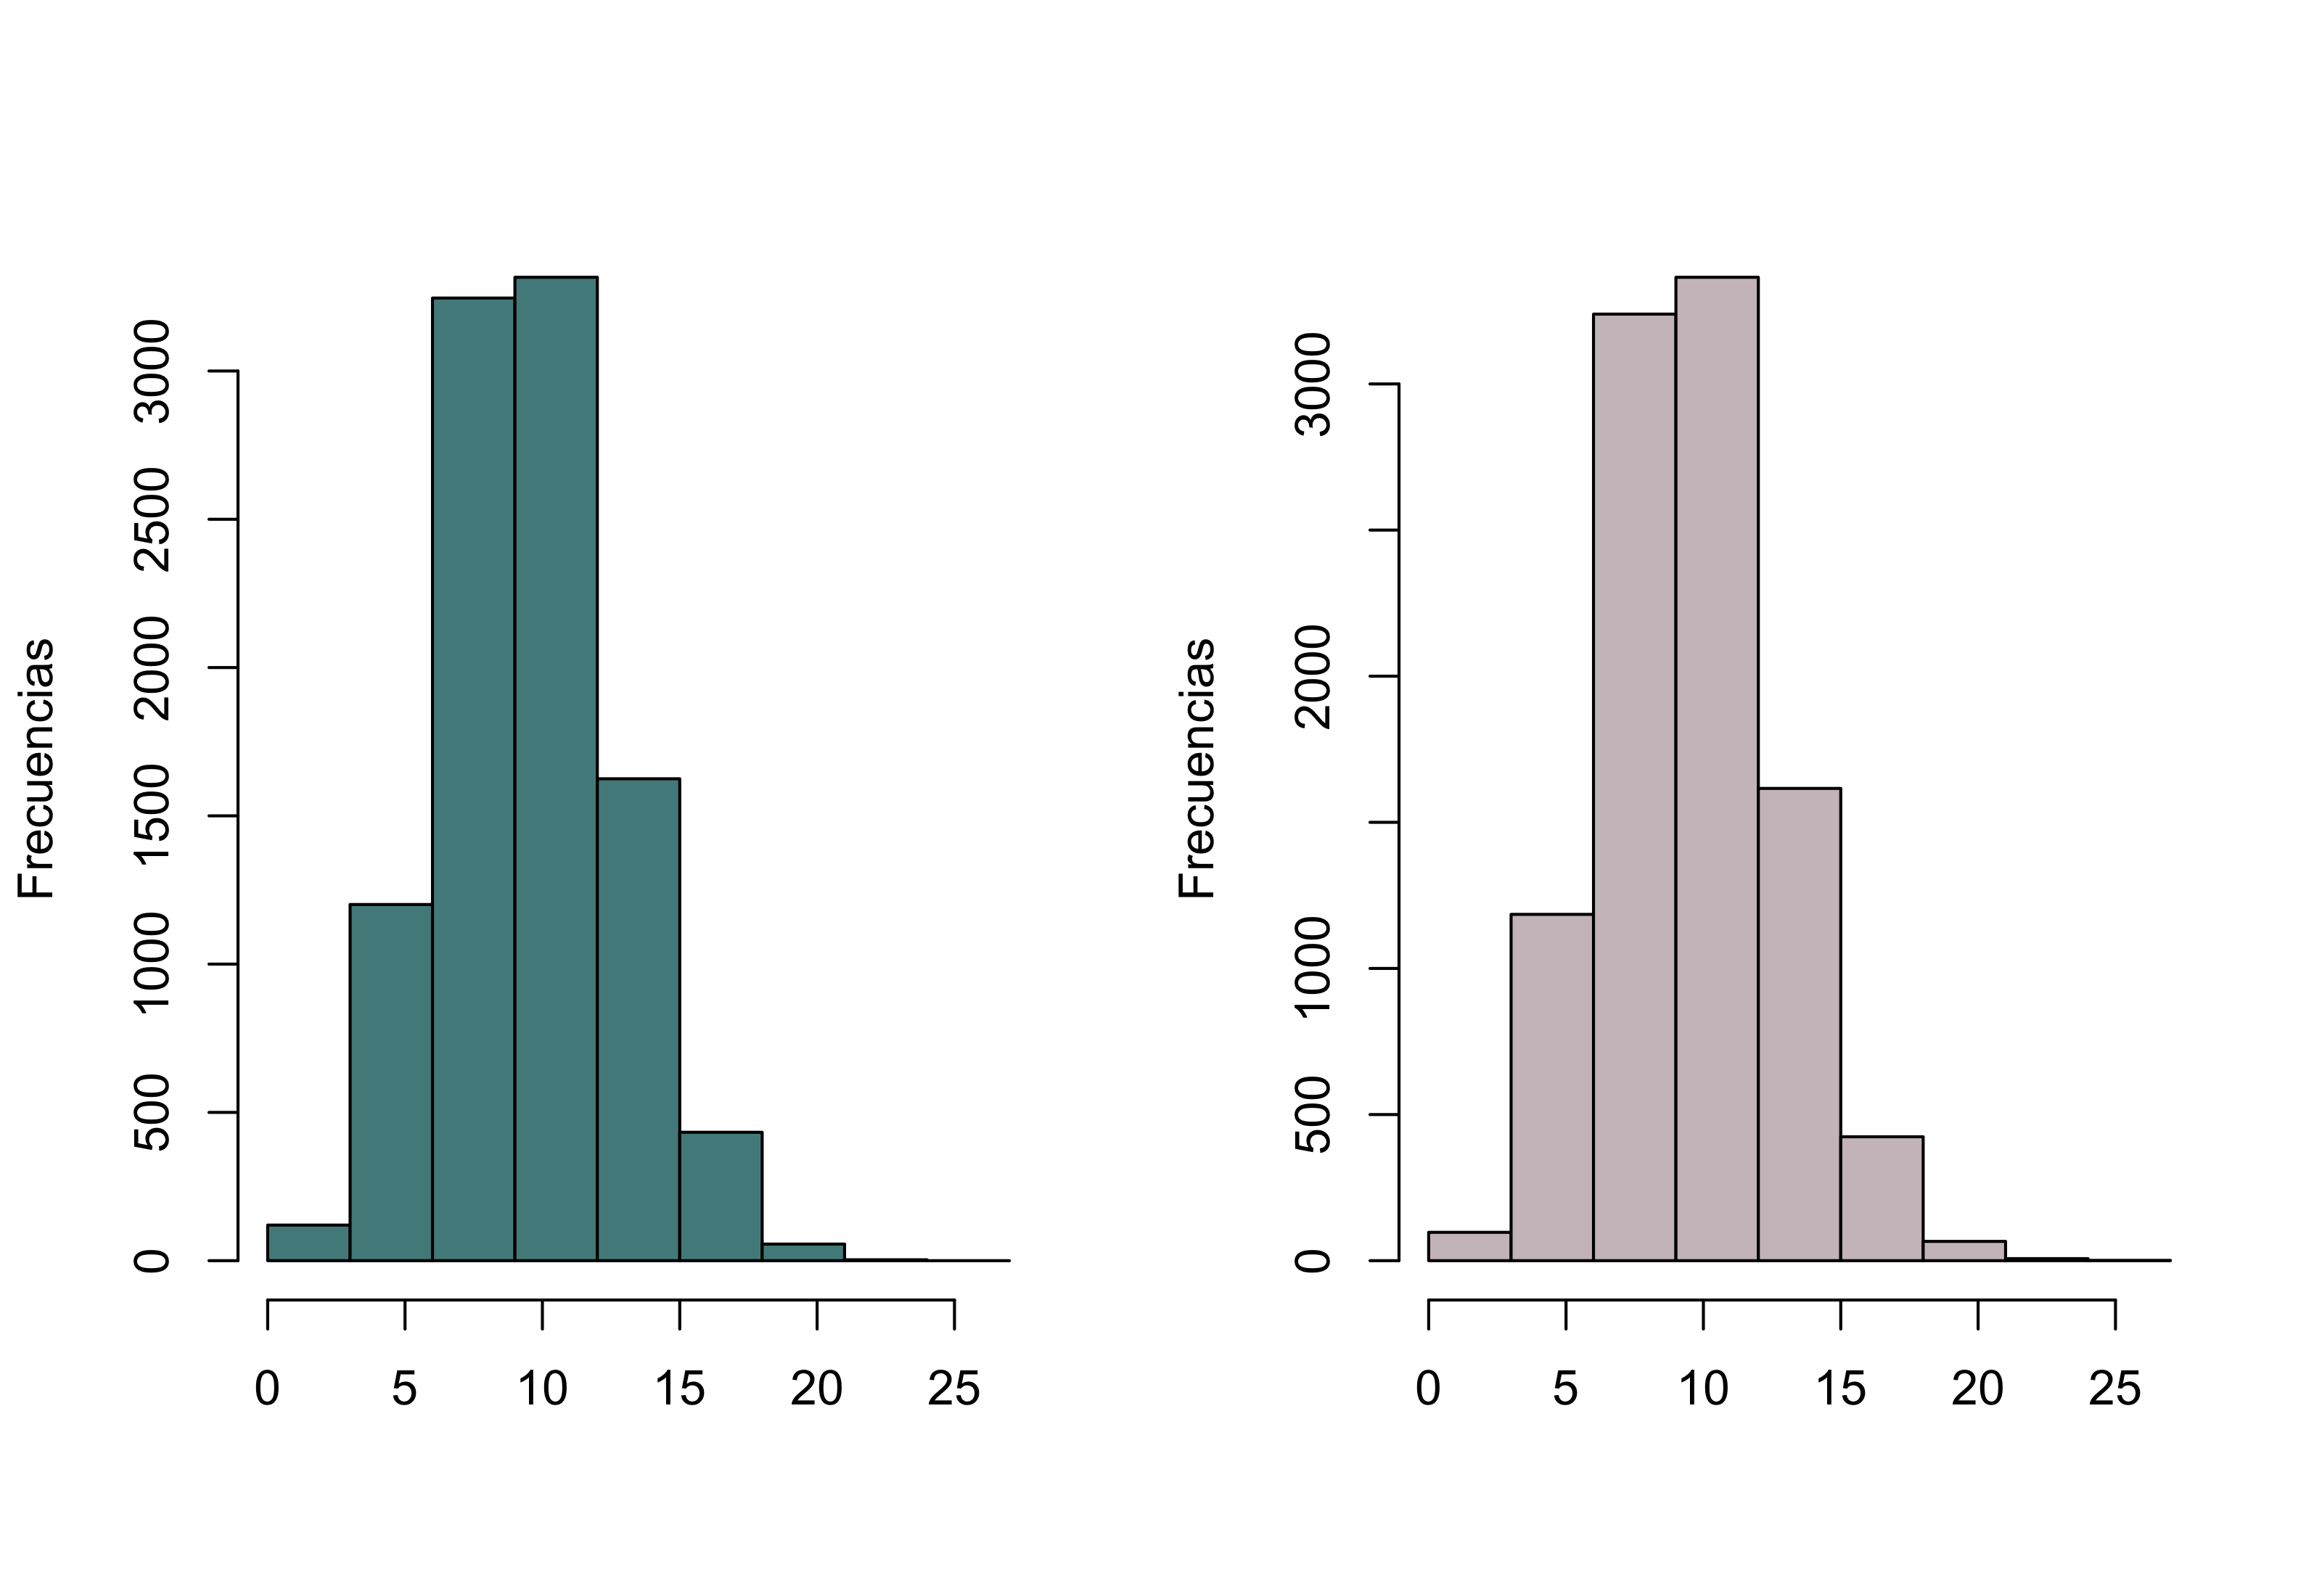
\includegraphics[width=\linewidth]{unif2.png} 		
 		\caption{Números generados con \texttt{lambda}=10 (izq) contra los generados con \texttt{rpois} (der).}
 		\label{pr2unif}
 	\end{subfigure}
 	 	\begin{subfigure}[b]{0.45\linewidth}
 		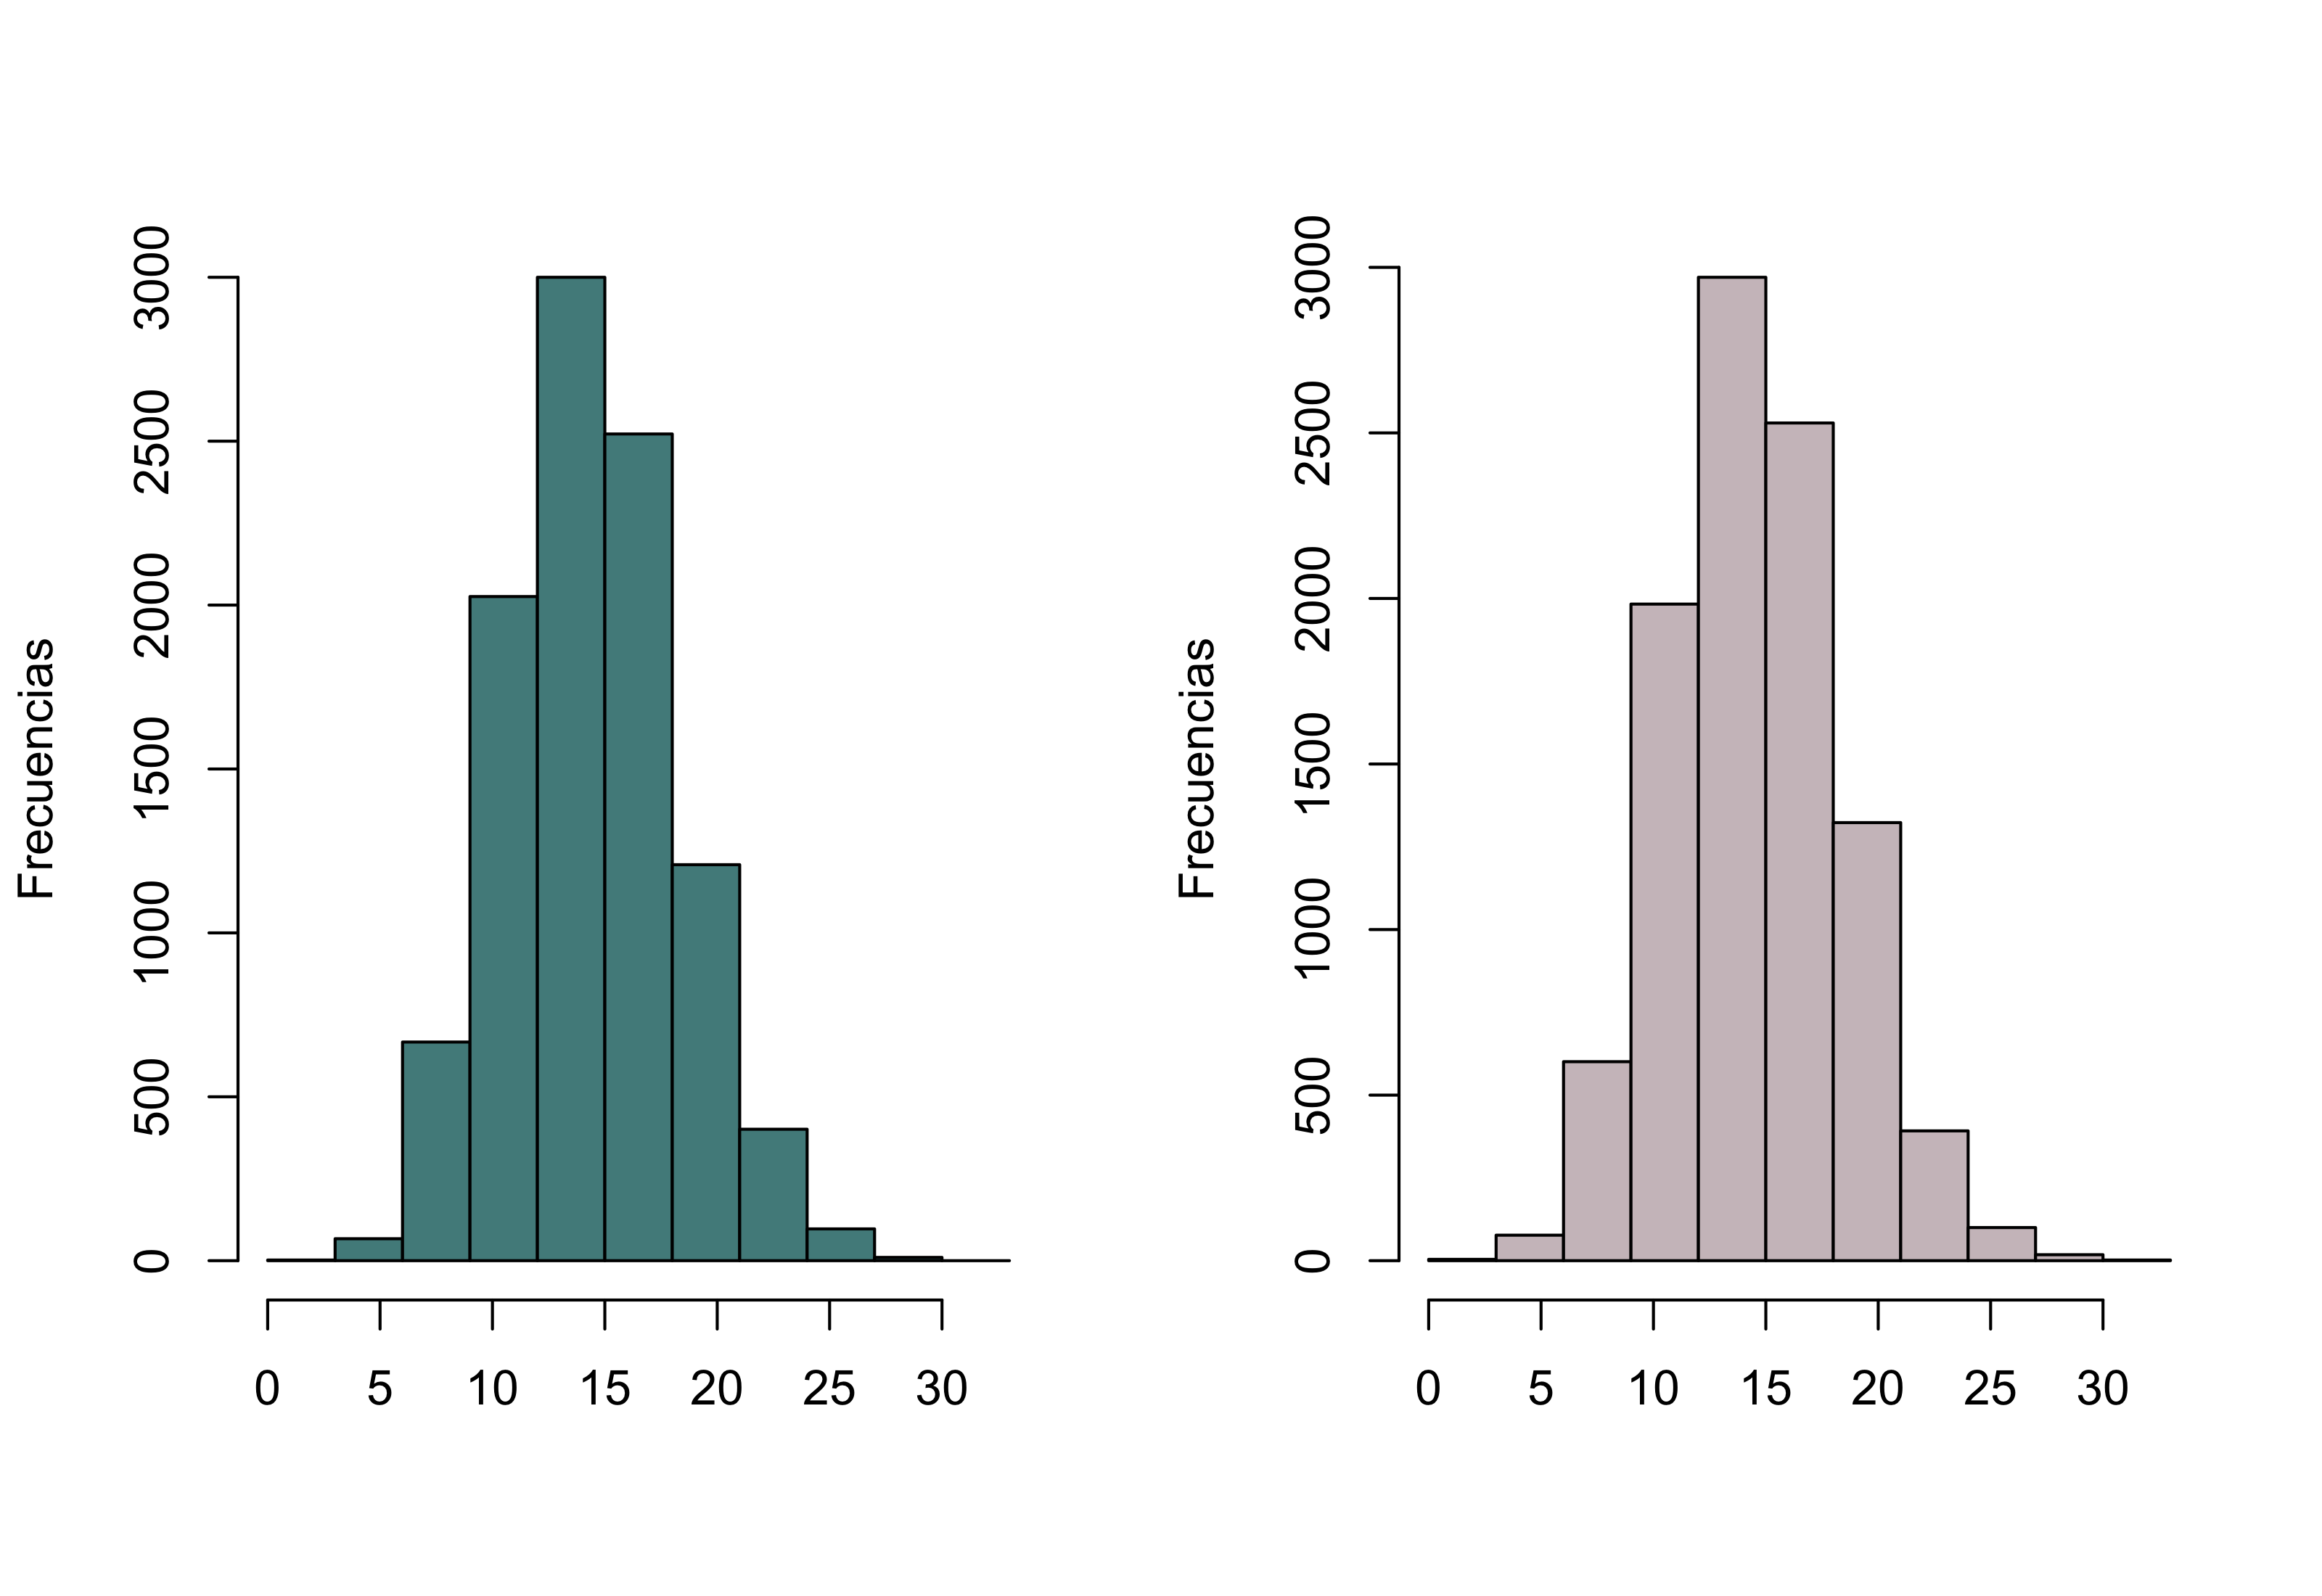
\includegraphics[width=\linewidth]{unif3.png} 		
 		\caption{Números generados con \texttt{lambda}=15 (izq) contra los generados con \texttt{rpois} (der).}
 		\label{pr3unif}
 	\end{subfigure}
 	 	\hfill
 	 	\begin{subfigure}[b]{0.45\linewidth}
 		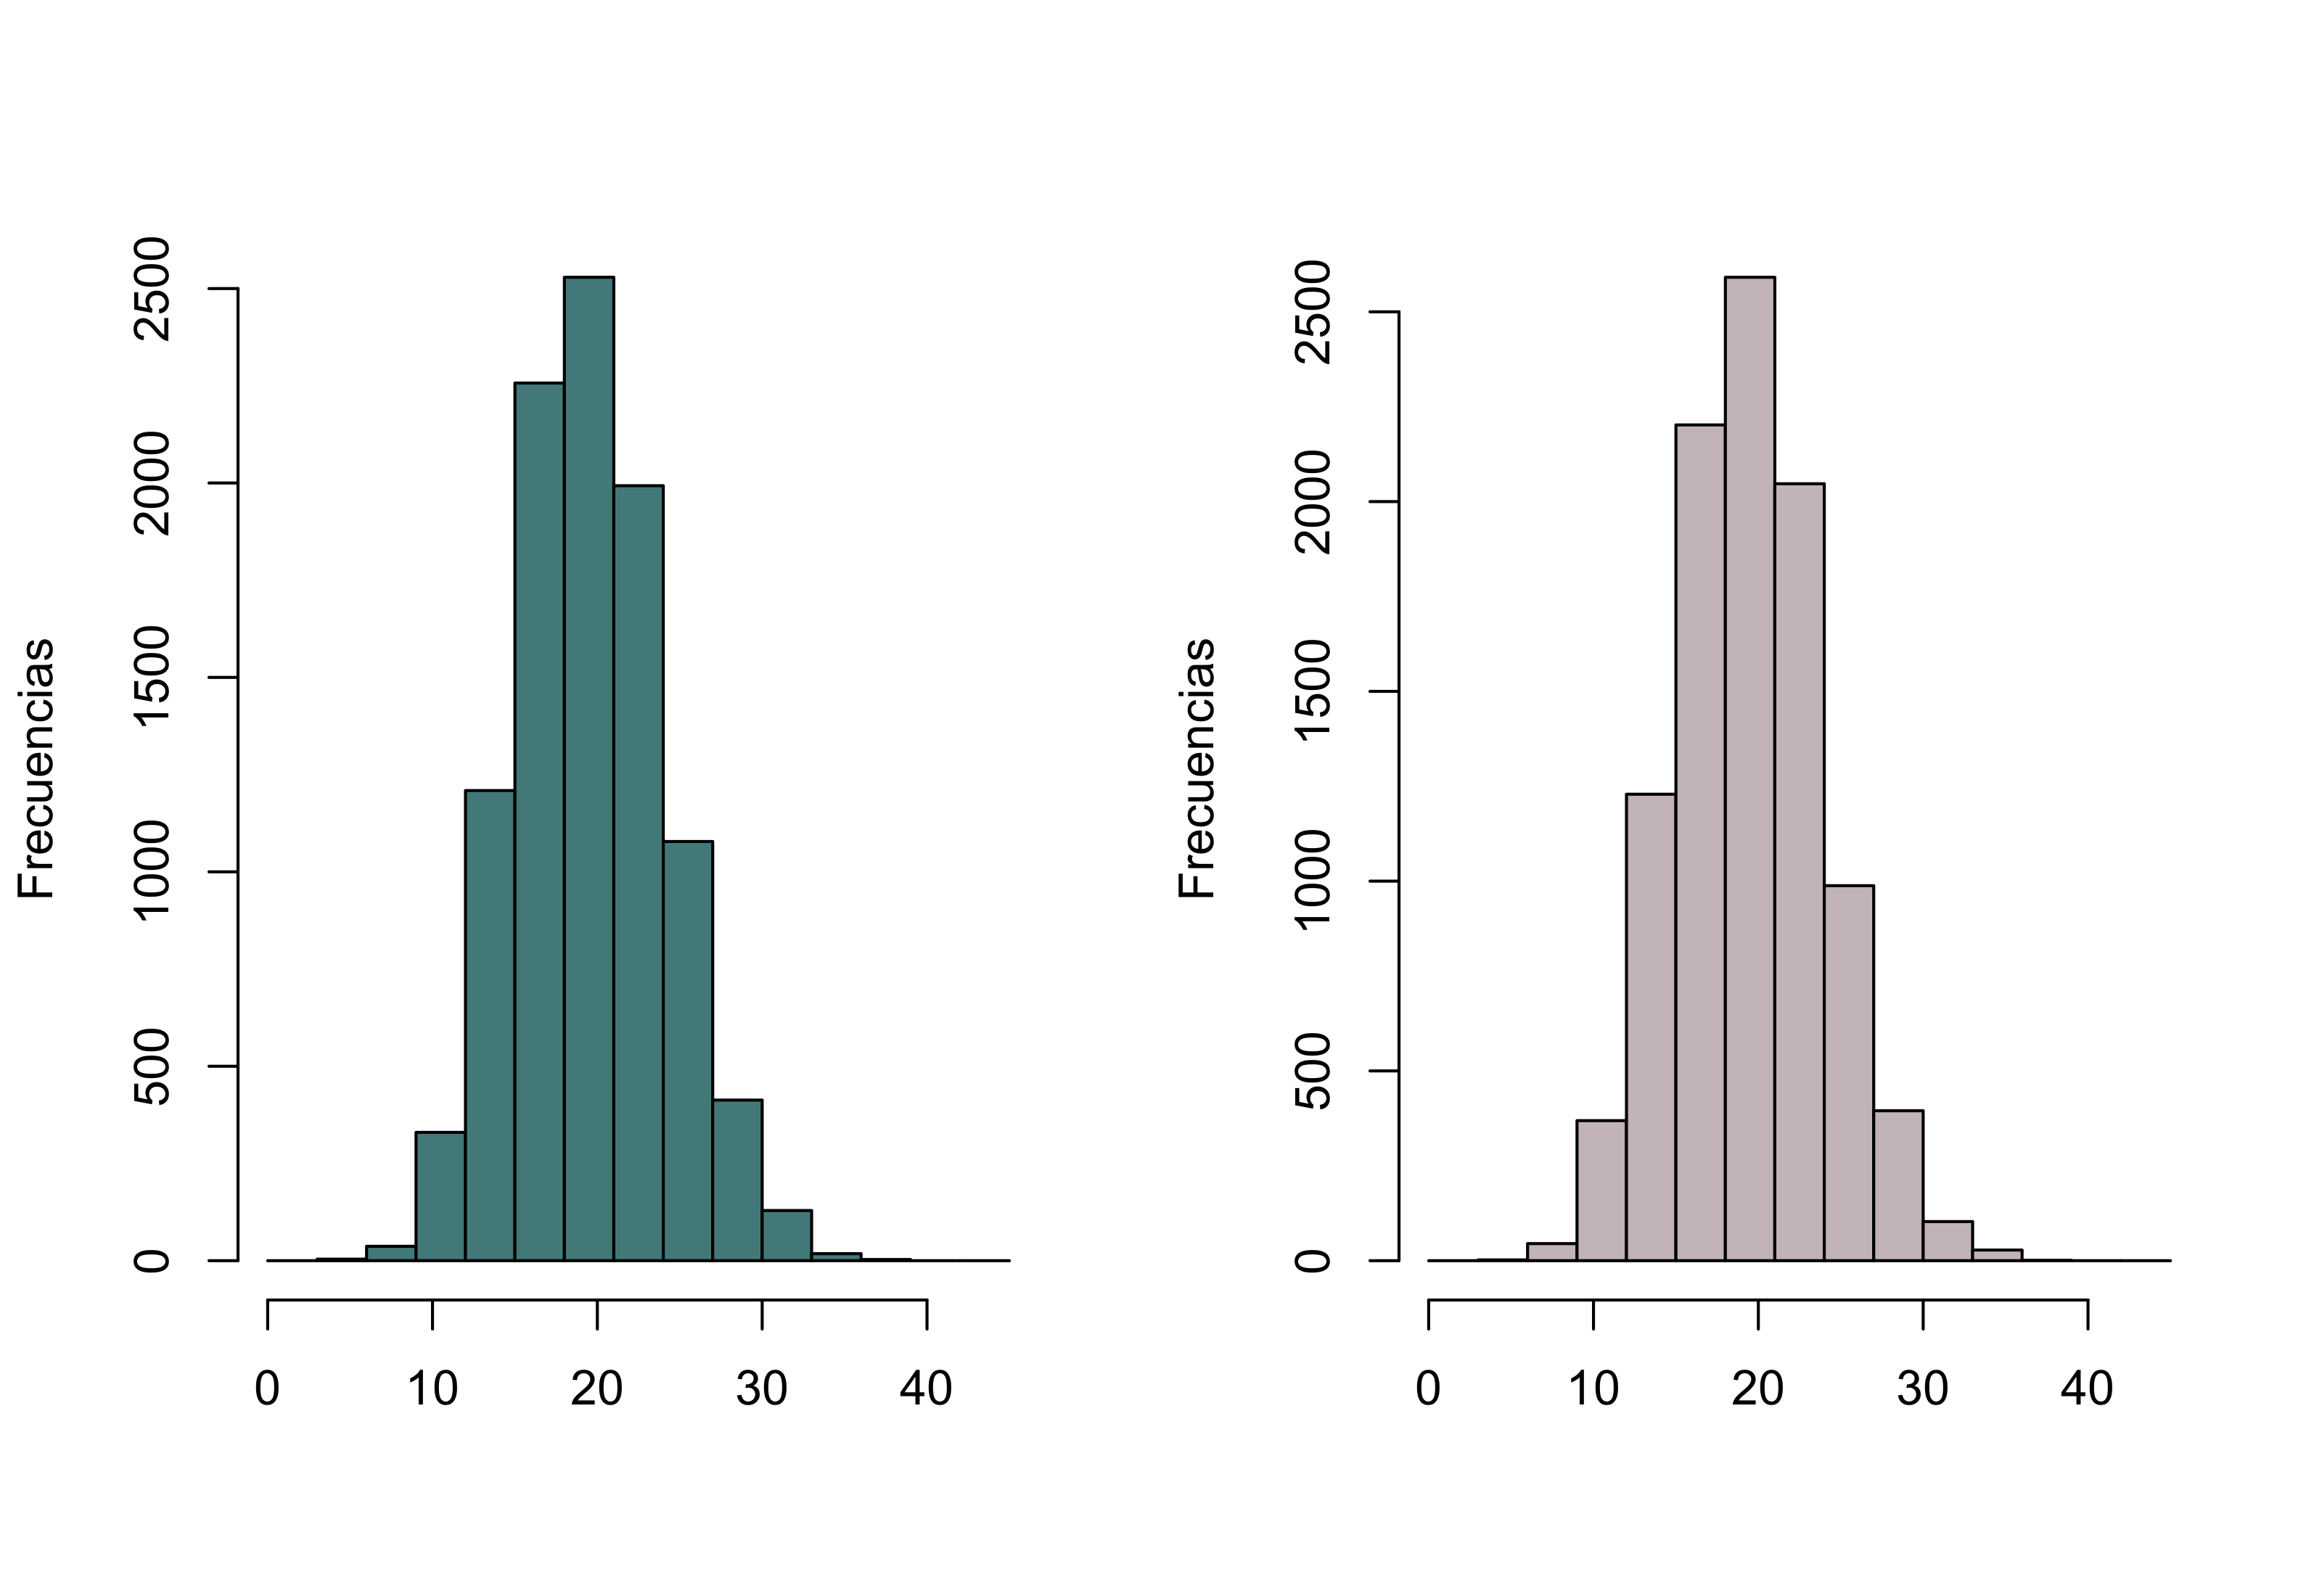
\includegraphics[width=\linewidth]{unif4.png} 		
 		\caption{Números generados con \texttt{lambda}=20 (izq) contra los generados con \texttt{rpois} (der).}
 		\label{pr4unif}
 	\end{subfigure}
 	 	\caption{Experimentos usando el algoritmo de Knuth.} 
 	 		\label{prsunif}
\end{figure}

\begin{table}
\centering
\caption{Comparación del lambda usado y el lambda dado por \texttt{goodfit}.}
\begin{tabular}{cccr}
\hline 
Prueba & Lambda & Lambda (goodfit) \\ 
\hline 
1 & 5 & 4.987 \\ 
2 & 10 & 10.009 \\ 
3 & 15 & 15.0388 \\ 
4 & 20 & 20.013 \\ 
\hline 
\end{tabular} 
\label{datosunif}
\end{table}

\section{Distribución de Poisson en el libro de texto}
Continuando con el estudio de la novela \textit{Alice's Adventures in Wonderland} \cite{alice}, se busca en qué tiempos aparece la palabra \texttt{Alice} y comparar su distribución con la de números generados con \texttt{rpois}.

Consideramos una unidad de tiempo como cien palabras. Se obtiene el promedio de eventos en una unidad de tiempo, es decir, en promedio cuantas veces aparece \texttt{Alice} en cien palabras. Se encuentra que dichos valores siguen una distribución de Poisson con $\lambda$ igual al promedio de los datos. En la figura \ref{libro} se muestra en la izquierda del histograma de los datos generados con el algoritmo y en la derecha el histograma de los números generados con \texttt{rpois}.

\begin{figure}
\centering	
	\begin{subfigure}[b]{0.45\linewidth}
 		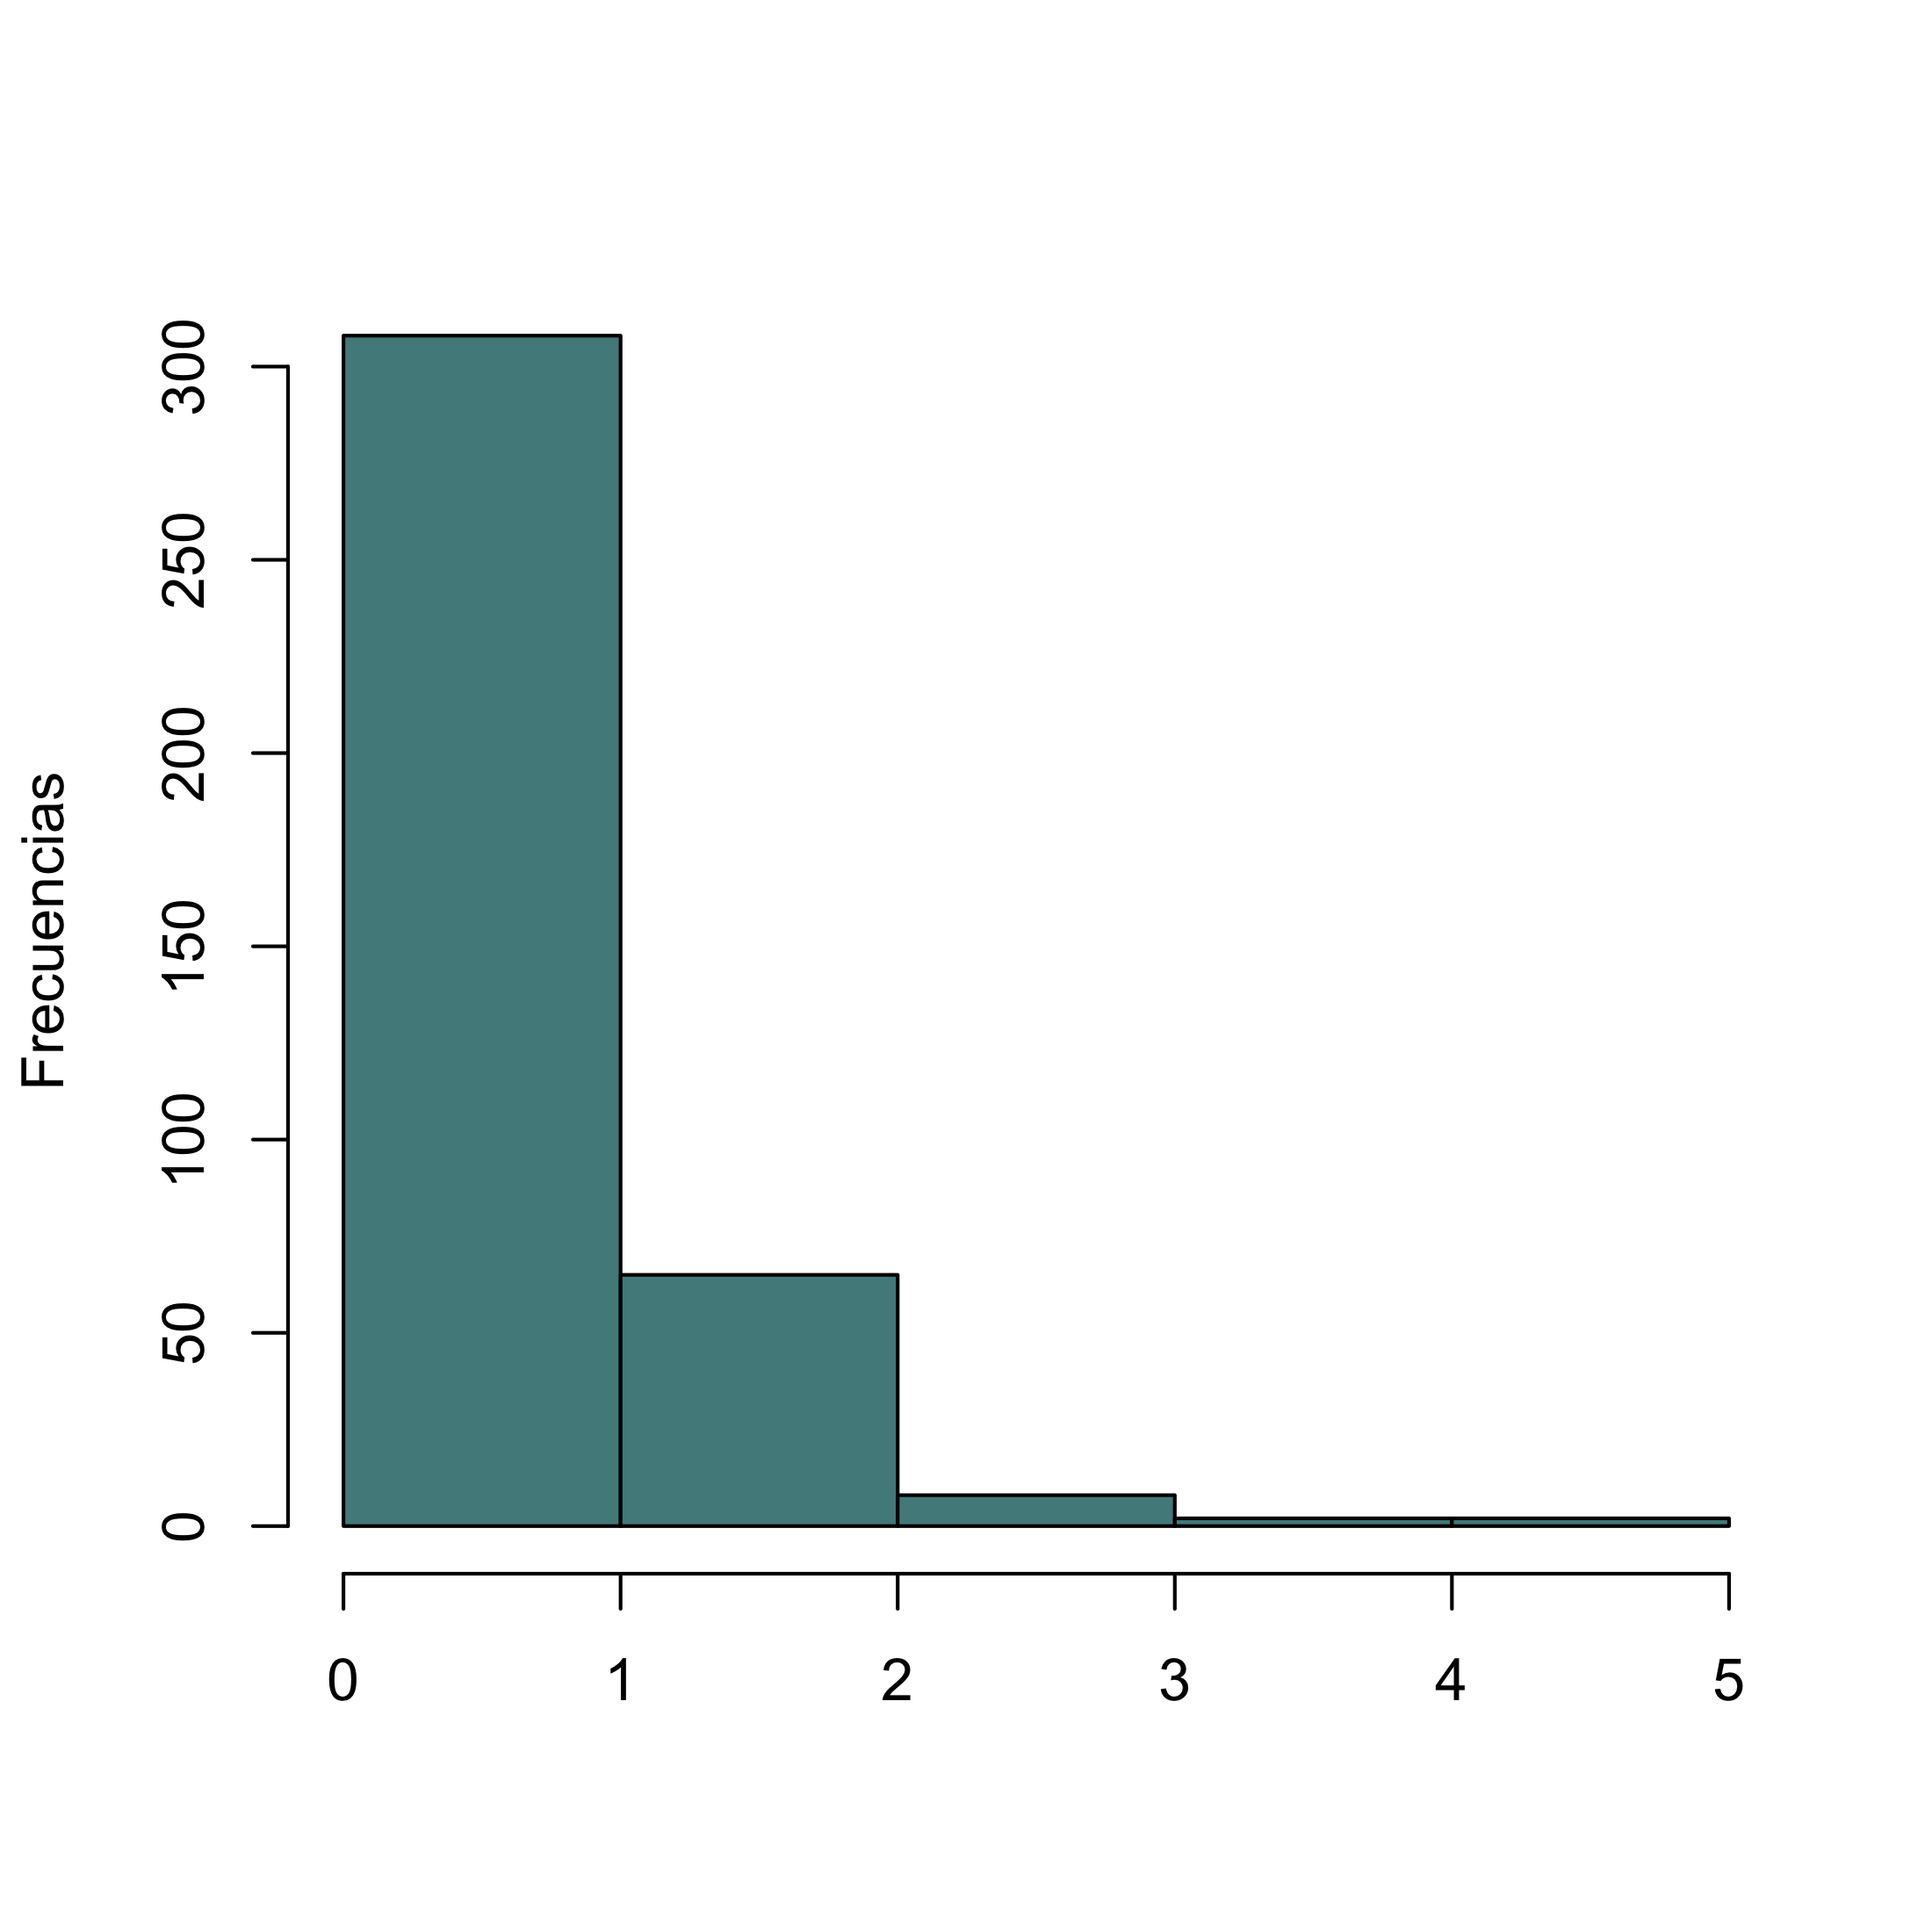
\includegraphics[width=\linewidth]{libroexp.png}
 		\caption{Diferencia entre los tiempos de aparición de la palabra \textit{Alice}.}
 		\label{alice}
	\end{subfigure}
	\begin{subfigure}[b]{0.45\linewidth}
 		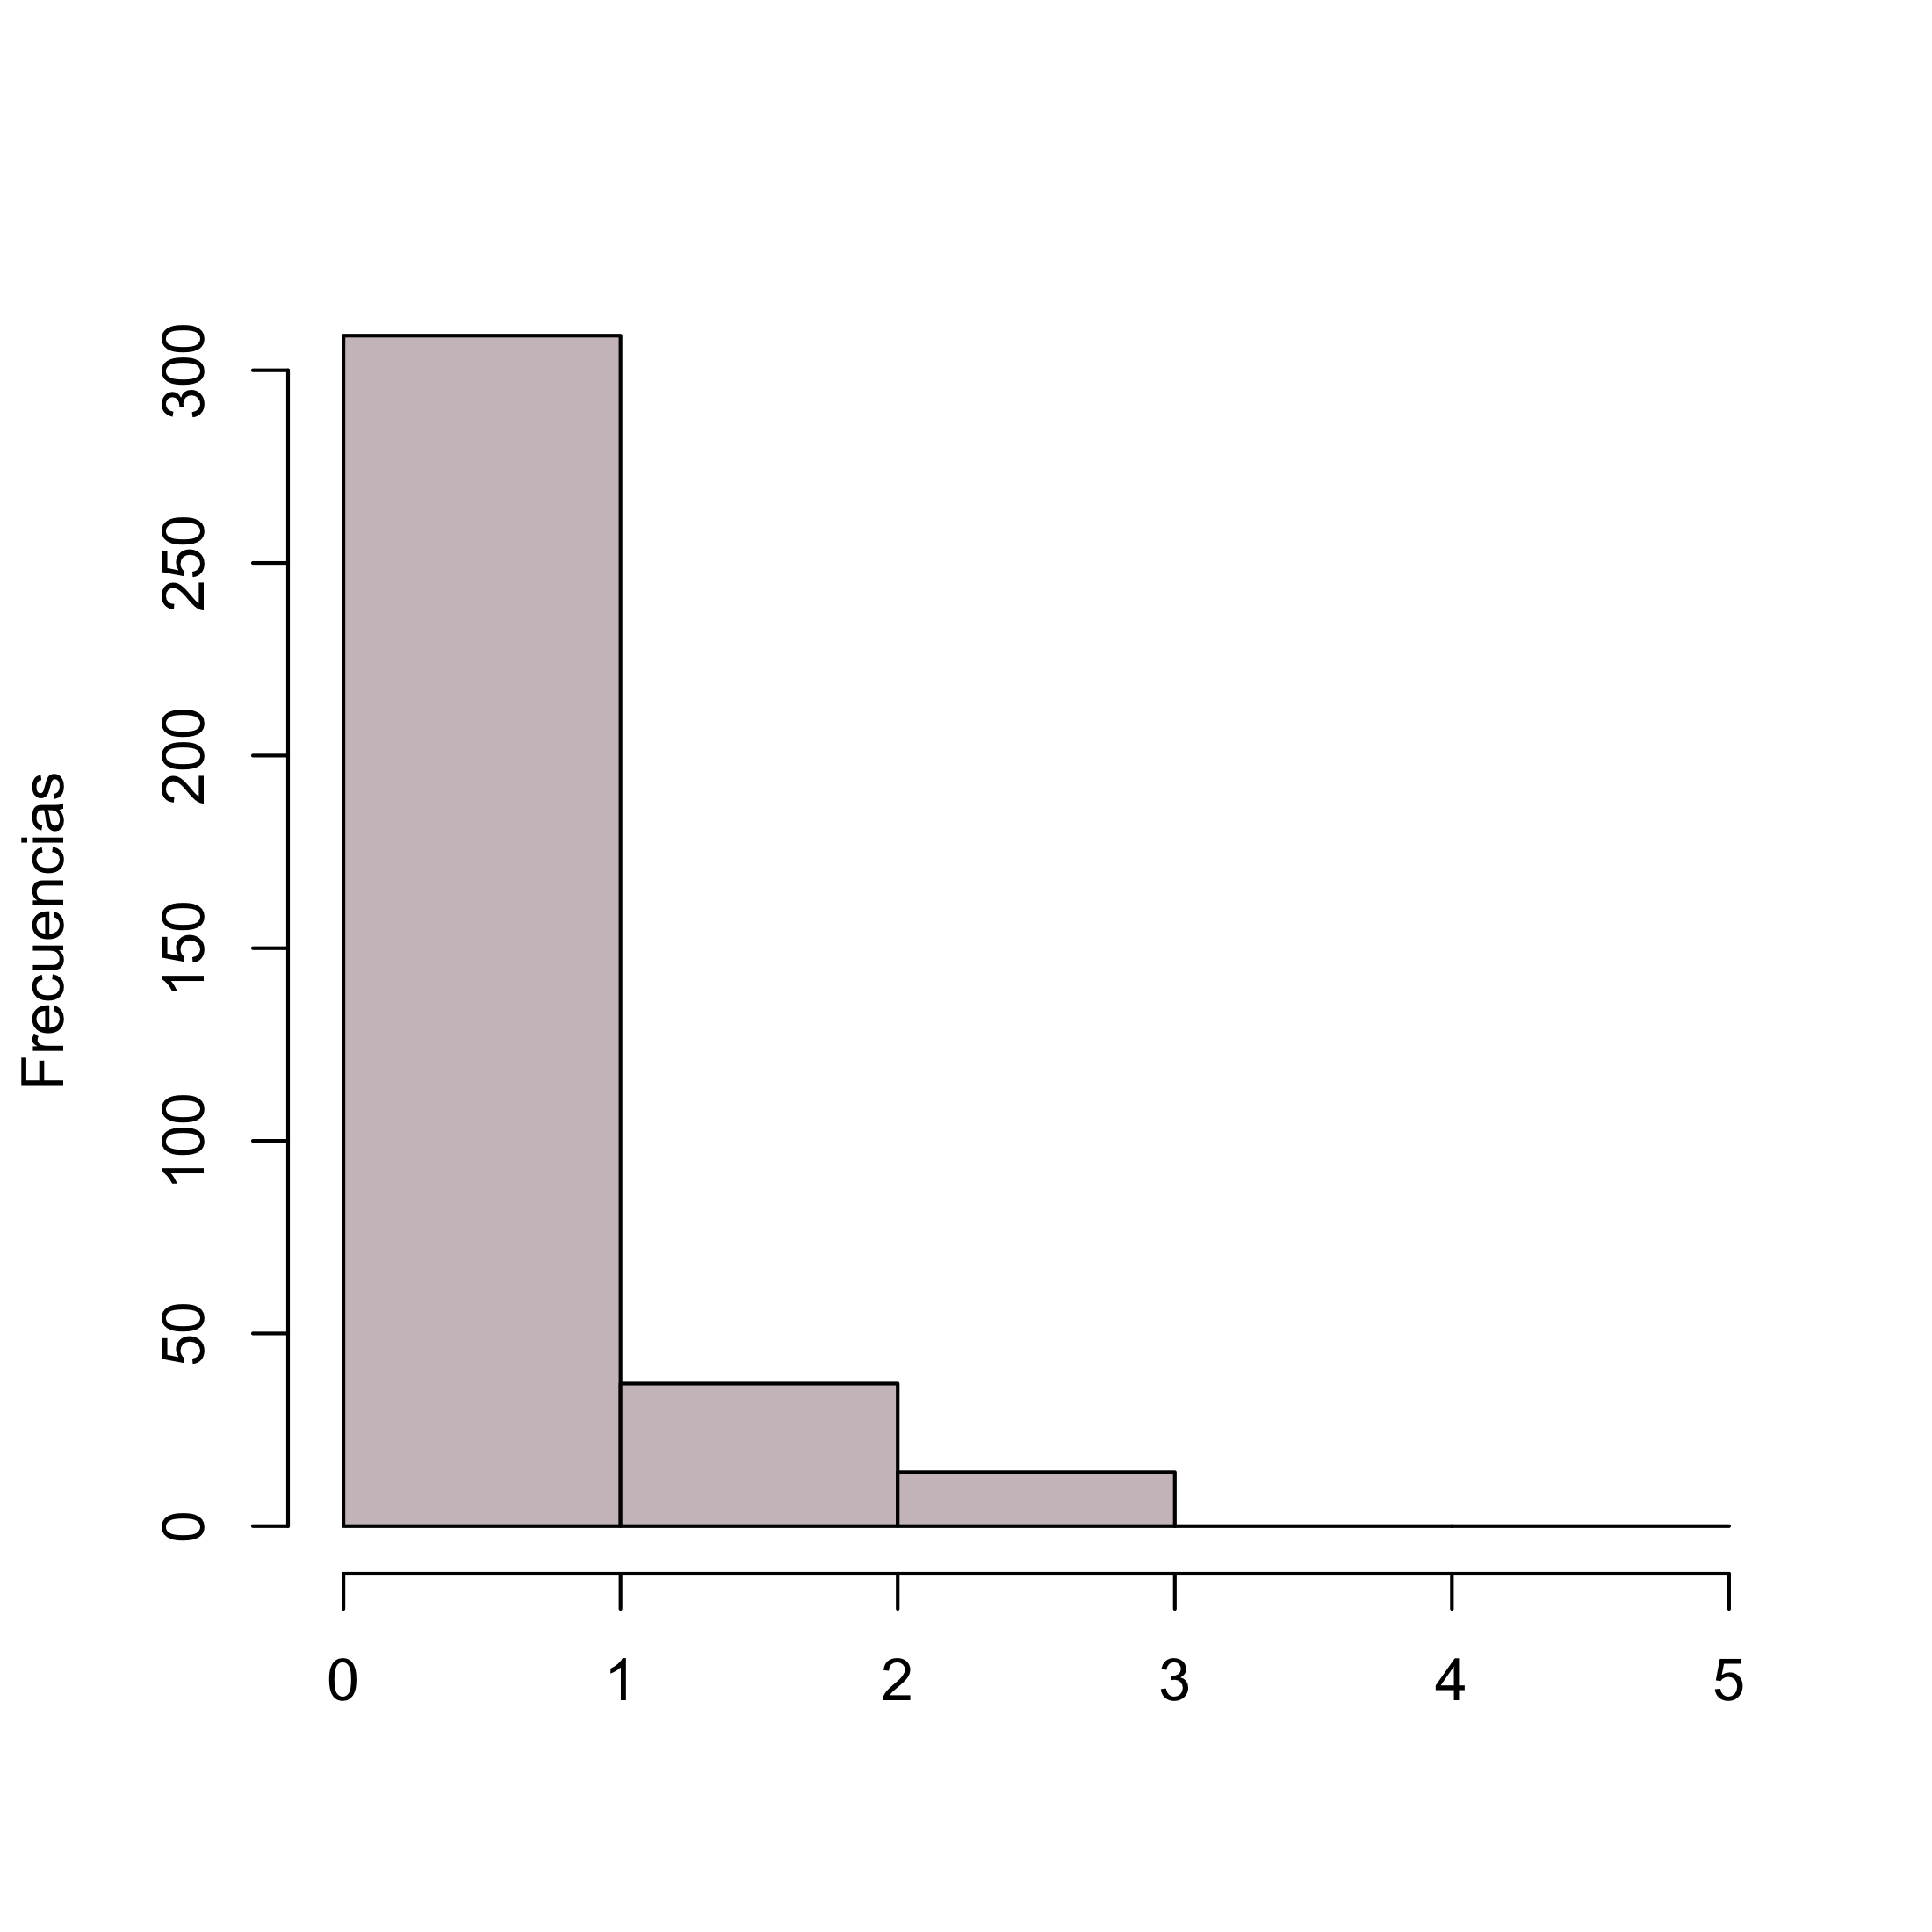
\includegraphics[width=\linewidth]{generadosexp.png}
 		\caption{Números generados con distribución Poisson.}
 	\label{generadoslibro}
	\end{subfigure}
	\caption{Tiempos entre apariciones de la palabra \textit{Alice}.}
		\label{libro}
	\end{figure}
\bibliographystyle{plain} 
\bibliography{Referencias}




\end{document}